\documentclass[../notes.tex]{subfiles}

\pagestyle{main}
\renewcommand{\chaptermark}[1]{\markboth{\chaptername\ \thechapter\ (#1)}{}}
\setcounter{chapter}{3}

\begin{document}




\chapter{Carboxylic Acids and Derivatives}
\setcounter{section}{22}
\section{Carboxylic Acids Intro}
\begin{itemize}
    \item \marginnote{10/30:}Lecture 22 recap.
    \begin{enumerate}[label={\Alph*.}]
        \item Amine synthesis by direct S\textsubscript{N}2 (of, for example, \ce{NH3}) leads to mixtures unless you use a very large excess of ammonia (Figure \ref{fig:amineAlkylationRX}).
        \begin{itemize}
            \item Alternative: Gabriel synthesis (Figure \ref{fig:gabrielSynthesis}).
            \item Alternative: Conversion of a primary or secondary alkyl halide to an azide and subsequent reduction (Figure \ref{fig:azideReduce}).
        \end{itemize}
        \item Reductive amination is an incredibly powerful technique (Figures \ref{fig:redAmin23}, \ref{fig:redAmin12}, \& \ref{fig:redAmin01}).
        \begin{itemize}
            \item It can build primary, secondary, and tertiary amines.
            \item Be intimately familiar with this process for Exam 3!!
        \end{itemize}
        \item Acylation/reduction is also a great method (Figure \ref{fig:acylReduce}).
        \begin{itemize}
            \item Acylate the amine to give an amide intermediate, reduce with LAH, and quench with water.
        \end{itemize}
        \item Primary and secondary alkyl bromides, iodides, and tosylates can be substituted to the nitrile and reduced to an amine (Figure \ref{fig:nitrileReducX}).
        \begin{itemize}
            \item This is a 1-carbon homologation.
        \end{itemize}
        \item HONO (generated from \ce{NaNO2 + HCl}) converts aniline to an aryl diazonium salt (Figure \ref{fig:diazoniumForm}).
    \end{enumerate}
    \item Announcement: The notes taken by the TFs are posted on Canvas (that's these!).
    \begin{itemize}
        \item Consider referring to these even over the ones that Prof. Buchwald provides.
    \end{itemize}
    \item Lecture 22 continued.
    \item Using the sequence of reaction in Figure \ref{fig:diazoniumBenz}, you can form an aryl diazonium salt.
    \begin{itemize}
        \item Treating it with \ce{KI} yields an aryl iodide.
        \item Treating it with \ce{H2O} yields a phenol.
        \item Treating it with hypophosphorus acid (\ce{H3PO2}) yields benzene again.
        \begin{itemize}
            \item Once again, you are not responsible for the name "hypophosphorus acid."
        \end{itemize}
        \item Treating it with \ce{CuX} (where $\ce{X}=\ce{Cl},\ce{Br},\ce{CN}$) yields \ce{PhX}.
    \end{itemize}
    \item This is a great example of what we do with synthesis!
    \begin{itemize}
        % \item Example: \emph{para}-bromoanisole maybe came from HONO followed by the aryl diazonium salt??
        \item Synthesis is all about connecting compounds with transformations.
        \item Breaking down the example in such a way is called \textbf{retrosynthetic analysis}.
    \end{itemize}
    \item Recall from last time that azides are reduced to amines by \ce{LiAlH4} and a subsequent water workup (Figure \ref{fig:azideReduce}). Here's a further note on this.
    \begin{figure}[H]
        \centering
        \footnotesize
        \schemestart
            \chemfig{*6(--(*3(<O>))----)}
            \arrow(c1--c23){0}[,2]
            \subscheme{
                \chemfig{*6(--(<OH)-(<:N_3)---)}
                \arrow(c2--c3){->[{[H]}]}[,1.4]
                \chemfig{*6(--(<OH)-(<:NH_2)---)}
                \arrow(@c2--c4){0}[-90,0.5]
                \chemfig{*6(--(<OH)-(<:CN)---)}
                \arrow(--c5){->[1. \ce{LiAlH4}][2. \ce{H2O}\hspace{3.6mm}\ ]}[,1.4]
                \chemfig{*6(--(<OH)-(<:-[:-30]NH_2)---)}
            }
        \schemestop
        \chemmove{
            \draw ([xshift=9pt]c1.east) -- ($(c1)!0.3!(c23)$) coordinate (c25) -- (c25 |- c2) -- node[above]{1. \ce{NaN3}} node[below]{2. \ce{H+}\hspace{3mm}\ } ([xshift=-9pt]c2.west);
            \draw (c25) -- (c25 |- c4) -- node[above]{1. \ce{NaCN}} node[below]{2. \ce{H+}\hspace{4mm}\ } ([xshift=-9pt]c4.west);
        }
        \caption{Aminoalcohol synthesis from epoxides.}
        \label{fig:aminoalcoholEpox}
    \end{figure}
    \begin{itemize}
        \item Recall from 5.12 that \textbf{epoxides} are essentialy just reactive ethers, due to their ring strain.
        \item Therefore, if we treat an epoxide with \ce{NaN3}, we'll get a backside attack that yields a certain intermediate.
        \item Then upon reduction, we get a \emph{trans}-1,2-aminoalcohol.
        \begin{itemize}
            \item This is an important functional group for $\beta$-blockers in biology!
        \end{itemize}
        \item Alternatively, we can treat epoxides with \ce{CN-}, yielding the cyanoalcohol.
        \begin{itemize}
            \item We can then reduce this to the 1,3-aminoalcohol.
        \end{itemize}
    \end{itemize}
    \item This concludes our discussion of amines.
    \item Today: Introduction to carboxylic acids and their derivatives.
    \begin{itemize}
        \item Reading: Chapter 10 of \textcite{bib:Clayden}.
    \end{itemize}
    \item Lecture outline.
    \begin{enumerate}
        \item Introduction.
        \item Synthesis of carboxylic acids.
        \begin{enumerate}[label={\alph*.}]
            \item Oxidation of alcohols and aldehydes.
            \item Carboxylation of Grignard reagents.
            \item Hydrolysis of nitriles.
            \item Types of carboxylic acid derivatives.
        \end{enumerate}
        \item Acyl transfer reactions.
        \begin{enumerate}[label={\alph*.}]
            \item Background.
        \end{enumerate}
    \end{enumerate}
    \item We'll begin with Topic 1: Introduction.
    \item \textbf{Carboxylic acid derivative}: A compound of the following form, where $\ce{X}\neq\ce{H},\ce{R}$. \emph{Structure}
    \begin{figure}[h!]
        \centering
        \footnotesize
        \chemfig{R-[:30](=[2]O)-[:-30]X}
        \caption{Carboxylic acid derivative.}
        \label{fig:carbDeriv}
    \end{figure}
    \begin{itemize}
        \item Since \ce{X} is \emph{not} equal to \ce{H} or \ce{R}, we're not considering aldehydes or ketones.
    \end{itemize}
    \pagebreak
    \item \textbf{Carboxylic acid}: A carboxylic acid derivative for which $\ce{X}=\ce{OH}$. \emph{Structure}
    \begin{figure}[h!]
        \centering
        \footnotesize
        \schemestart
            \chemfig{R-[:30](=[2]O)-[:-30]OH}
            \arrow{<=>[][\ce{H+}]}
            \chemleft{[}\subscheme{
                \chemfig{R-[:30](=[2]O)-[:-30]\charge{45=$\ominus$}{O}}
                \arrow{<->}
                \chemfig{R-[:30](=[:-30]O)-[2]\charge{45=$\ominus$}{O}}
            }\chemright{]}
            \arrow{0[\small$\equiv$][][-2mm]}
            \chemfig{R-[:30]\charge{[extra sep=8pt]30=$\ominus$}{}(-[2]@{Ot}O)-[:-30]@{Ob}O}
        \schemestop
        \chemmove{
            \draw [densely dashed,-,shorten <=7pt,shorten >=7pt] ($(Ot)+(30:0.05)$) to[bend right=30,looseness=1.2] ($(Ob)+(30:0.05)$);
        }
        \caption{Carboxylic acid.}
        \label{fig:carbAcid}
    \end{figure}
    \begin{itemize}
        \item $\pKa\approx 5$.
        \begin{itemize}
            \item By comparison, $\pKa\approx 16$ for an alcohol.
            \item Therefore, carboylic acids are \emph{eleven orders of magnitude} more acidic than alcohols.
        \end{itemize}
        \item Deprotonation gives us a resonance-stabilized \textbf{carboxylate}, which can be drawn either as resonance forms or as a delocalized anion.
    \end{itemize}
    \item One of the simplest carboxylic acids is \textbf{acetic acid}.
    \item \textbf{Acetic acid}: The carboxylic acid for which $\ce{R}=\ce{Me}$. \emph{Structure}
    \begin{figure}[h!]
        \centering
        \footnotesize
        \chemfig{H_3C-[:30](=[2]O)-[:-30]OH}
        \caption{Acetic acid.}
        \label{fig:aceticAcid}
    \end{figure}
    \begin{itemize}
        \item Acetic acid is in vinegar! In fact, vinegar is about 4-5\% acetic acid in water.
        \item Acetic acid is also used as an industrial solvent (in the 100\% pure form, which is quite caustic).
        \item How is acetic acid made?
        \begin{equation*}
            \ce{MeOH ->[CO][cat] CH3COOH}
        \end{equation*}
        \begin{itemize}
            \item Acetic acid is produced industrially via the Monsanto acetic acid process, which carries out the carbonylation of methanol using a rhodium catalyst.
        \end{itemize}
    \end{itemize}
    \item The first several biscarboxylic acids.
    \begin{figure}[h!]
        \centering
        \footnotesize
        \begin{subfigure}[b]{0.25\linewidth}
            \centering
            \chemfig{HO_2C-CO_2H}
            \caption{Oxalic acid.}
            \label{fig:biscarboxylica}
        \end{subfigure}
        \begin{subfigure}[b]{0.25\linewidth}
            \centering
            \chemfig{HO_2C-[:30]-[:-30]CO_2H}
            \caption{Malonic acid.}
            \label{fig:biscarboxylicb}
        \end{subfigure}
        \begin{subfigure}[b]{0.25\linewidth}
            \centering
            \chemfig{HO_2C-[:60]--[:-60]CO_2H}
            \caption{Succinic acid.}
            \label{fig:biscarboxylicc}
        \end{subfigure}\\[2em]
        \begin{subfigure}[b]{0.25\linewidth}
            \centering
            \chemfig{HO_2C-[2,,3]-[:30]-[:-30]-[6]CO_2H}
            \caption{Glutaric acid.}
            \label{fig:biscarboxylicd}
        \end{subfigure}
        \begin{subfigure}[b]{0.25\linewidth}
            \centering
            \chemfig{HO_2C-[:120,,3]-[::-60]-[::-60]-[::-60]-[::-60,,,1]CO_2H}
            \caption{Adipic acid.}
            \label{fig:biscarboxylice}
        \end{subfigure}
        \begin{subfigure}[b]{0.25\linewidth}
            \centering
            \chemfig{HO_2C-[3,,3]-[2,1.2]-[::-60,1.4]-[::-60,1.4]-[::-60,1.2]-[5,,,1]CO_2H}
            \caption{Pimelic acid.}
            \label{fig:biscarboxylicf}
        \end{subfigure}
        \caption{Biscarboxylic acids.}
        \label{fig:biscarboxylic}
    \end{figure}
    \begin{itemize}
        \item \textbf{Oxalic}, \textbf{malonic}, \textbf{succinic}, \textbf{glutaric}, \textbf{adipic}, and \textbf{pimelic} acids.
        \item Aside: Adipic acid is really important because it's involved in the manufacture of nylon.
        \item How do you remember all these names? There's a neumonic: OMSGAP or "Oh My, Such Good Apple Pie."
    \end{itemize}
    \item We now move onto Topic 2: Synthesis of carboxylic acids.
    \item Aside: A new definition of \textbf{oxidation} and \textbf{reduction}.
    \begin{itemize}
        \item Notice that in a carboxylic acid (e.g., see Figure \ref{fig:aceticAcid}), the central carbon has 3 bonds to oxygen.
        \item In contrast, a primary alcohol's central carbon has 1 bond to oxygen.
        \begin{itemize}
            \item Thus, we need to do a 4-electron oxidation to turn an alcohol into a carboxylic acid.
        \end{itemize}
        \item An aldehyde's central carbon has 2 bonds to oxygen.
        \begin{itemize}
            \item Thus, we need to do a 2-electron oxidation to turn an aldehyde into a carboxylic acid.
        \end{itemize}
        \item \ce{CO2}'s central carbon has 4 bonds to oxygen.
        \begin{itemize}
            \item Thus, we need to do a 2-electron reduction to turn \ce{CO2} into a carboxylic acid.
        \end{itemize}
        \item This array of related compounds motivates the following two definitions.
    \end{itemize}
    \item \textbf{Oxidation}: A chemical reaction that increases the number of carbon-oxygen bonds.
    \item \textbf{Reduction}: A chemical reaction that decreases the number of carbon-oxygen bonds.
    \item We now discuss Subtopic 2.a{}: Oxidation of alcohols and aldehydes.
    \begin{figure}[h!]
        \centering
        \footnotesize
        \begin{subfigure}[b]{0.57\linewidth}
            \centering
            \schemestart
                \chemfig{R-[:30]-[:-30]OH}
                \arrow{->[\ce{H2SO4}][\ce{CrO3}]}[,1.2]
                \chemleft{[}
                    \chemfig{R-[:30](=[2]O)-[:-30]H}
                \chemright{]}
                \arrow[,1.2]
                \chemfig{R-[:30](=[2]O)-[:-30]OH}
            \schemestop
            \caption{Primary alcohol or aldehyde to carboxylic acid.}
            \label{fig:OxAlcAlda}
        \end{subfigure}
        \begin{subfigure}[b]{0.42\linewidth}
            \centering
            \schemestart
                \chemfig{R-[:30]-[:-30]OH}
                \arrow{->[PCC]}[,1.2]
                \chemfig{R-[:30](=[2]O)-[:-30]H}
            \schemestop
            \caption{Primary alcohol to aldehyde.}
            \label{fig:OxAlcAldb}
        \end{subfigure}
        \caption{Oxidation of alcohols and aldehydes.}
        \label{fig:OxAlcAld}
    \end{figure}
    \begin{itemize}
        \item Suppose you have a primary alcohol.
        \begin{itemize}
            \item To convert it into a carboxylic acid, treat it with \textbf{Jones reagent}.
            \begin{itemize}
                \item The mechanism proceeds through the aldehyde.
                \item However, it can't stop, so it goes all the way to carboylic acid.
            \end{itemize}
            \item To stop the oxidation at the aldehyde, use PCC!
        \end{itemize}
        \item Now suppose you're starting at the aldehyde.
        \begin{itemize}
            \item To convert it to the carboxylic acid, just subject it to Jones reagent conditions! This is like picking up in the middle of the Figure \ref{fig:OxAlcAlda} mechanism.
        \end{itemize}
        \item Relevant reading: \textcite[194-196]{bib:Clayden}.
    \end{itemize}
    \item \textbf{Jones reagent}: The combination of excess \ce{H2SO4} and \ce{CrO3}.
    \item We now discuss Subtopic 2.b{}: Carboxylation of Grignard\footnote{"GRIN-yurd"} reagents.
    \begin{figure}[h!]
        \centering
        \footnotesize
        \schemestart
            \chemfig{R-Br}
            \arrow{->[\ce{Mg}]}
            \chemfig{R-MgBr}
            \arrow{->[\ce{CO2}]}
            \chemfig{R-[:30](=[2]O)-[:-30]\charge{45=$\ominus$}{O}}
            \arrow{->[\ce{H+}]}
            \chemfig{R-[:30](=[2]O)-[:-30]OH}
        \schemestop
        \caption{Carboxylation of Grignard reagents.}
        \label{fig:GrignardCO2}
    \end{figure}
    \pagebreak
    \begin{itemize}
        \item To make a Grignard reagent, react an alkyl bromide with magnesium.
        \begin{itemize}
            \item Aside (chemis-tea): Victor Grignard won the Nobel Prize for Grignard reagents, even though his mentor invented them!
            \item Note that Grignard reagents are very reactive! They are strong bases and strong nucleophiles, so if there's an acidic hydrogen in solution, it will get deprotonated.
            \begin{itemize}
                \item Essentially, we have to consider the functional group tolerance of a method.
            \end{itemize}
            \item These reactions are fun to do in the lab!
        \end{itemize}
        \item Once you make the Grignard reagent, just throw dry ice (a source of \ce{CO2}) into the flask. There will be a bunch of bubbling, and we'll get our carboxylic acid.
    \end{itemize}
    \item We now discuss Subtopic 2.c{}: Hydrolysis of nitriles.
    \begin{figure}[h!]
        \centering
        \footnotesize
        \schemestart
            \chemfig{R-CN}
            \arrow{->[{[O]}]}
            \chemfig{R-[:30](=[2]O)-[:-30]OH}
        \schemestop
        \caption{Nitrile hydrolysis.}
        \label{fig:nitrileHydro}
    \end{figure}
    \begin{itemize}
        \item Two ways to do this.
        \begin{itemize}
            \item Acid (\ce{H3O+}) and heat ($\Delta$).
            \item Base (\ce{HO-}), water (\ce{H2O}), and heat ($\Delta$) followed by quenching with acid and heat.
        \end{itemize}
        \item Nitriles are \emph{really, really, really} good intermediates (hint for Exam 3!!).
    \end{itemize}
    \item We'll now look at how nitriles may come up in a typical test question.
    \item Typical test question (TTQ): Provide two ways to convert benzyl bromide into phenylacetic acid.
    \begin{figure}[h!]
        \centering
        \footnotesize
        \schemestart
            \chemfig{Ph-[:30]-[:-30]Br}
            \arrow(c1--){->[*{0}\ce{Mg}]}[-45]
            \chemfig{Ph-[:30]-[:-30]MgBr}
            \arrow{->[1. \ce{CO2}][2. \ce{H+}\hspace{1.5mm}\ ]}[,1.4]
            \chemfig{Ph-[:30]-[:-30]CO_2H}
            \arrow(@c1--){->[*{0.0}\ce{NC-}]}[-135]
            \chemfig{Ph-[:30]-[:-30]CN}
            \arrow{->[Hydrolyse]}[180,1.4]
            \chemfig{Ph-[:30]-[:-30]CO_2H}
        \schemestop
        \caption{Typical test question: Multiple synthetic paths.}
        \label{fig:TTQmultSynth}
    \end{figure}
    \begin{itemize}
        \item First way: Make the Grignard and add \ce{CO2}.
        \item Second way: Do an S\textsubscript{N}2 with \ce{CN-}, and then hydrolyze the nitrile.
        \item Note that Prof. Buchwald uses checkmarks to denote the product on the board.\footnote{For an example of how this might look, see Figure \ref{fig:TTQnitrileKetoneb}.}
    \end{itemize}
    \item If we're answering a test question like this, will you want two separate arrows, or is one arrow with "1. \emph{reagent}" above and "2. \emph{reagent}" below?
    \begin{itemize}
        \item Either is good.
    \end{itemize}
    \item We now discuss Subtopic 2.d{}: Types of carboxylic acid derivatives.
    \item \textbf{Acid chloride}: A carboxylic acid derivative for which $\ce{X}=\ce{Cl}$. \emph{Structure}
    \begin{figure}[H]
        \centering
        \footnotesize
        \chemfig{R-[:30](=[2]O)-[:-30]Cl}
        \caption{Acid chloride.}
        \label{fig:carbAcidCl}
    \end{figure}
    \begin{itemize}
        \item These are far more common than acid bromides or acid iodides.\footnote{Coincidentally, acid iodides are used in the Monsanto acetic acid process!}
        \item To convert a carboxylic acid into an acid chloride, use \ce{SOCl2} and pyridine.\footnote{See the 5.12 equation review sheet!!}
        \item Mechanism: \textcite[214-215]{bib:Clayden}.
    \end{itemize}
    \item \textbf{Acid anhydride}: A carboxylic acid derivative for which $\ce{X}=\ce{RCO2}$. \emph{Structure}
    \begin{figure}[h!]
        \centering
        \footnotesize
        \chemfig{R-[:30](=[2]O)-[:-30]O-[:30](=[2]O)-[:-30]R}
        \caption{Acid anhydride.}
        \label{fig:carbAcidAnh}
    \end{figure}
    \begin{itemize}
        \item Synthesize these from two carboylic acids that combine and release water.
    \end{itemize}
    \item Example of an acid anhydride: Phthalic anhydride.
    \begin{figure}[h!]
        \centering
        \footnotesize
        \chemfig{*6(-=(*5(-(=O)-O-(=O)-))-=-=)}
        \caption{Phthalic anhydride.}
        \label{fig:phthalicAnhydride}
    \end{figure}
    \item \textbf{Ester}: A carboxylic acid derivative for which $\ce{X}=\ce{OR$'$}$. \emph{Structure}
    \begin{figure}[h!]
        \centering
        \footnotesize
        \chemfig{R-[:30](=[2]O)-[:-30]OR'}
        \caption{Ester.}
        \label{fig:carbEster}
    \end{figure}
    \begin{itemize}
        \item Esters are common in scents and smells.
    \end{itemize}
    \item Example of an ester: Isoamyl acetate.
    \begin{figure}[h!]
        \centering
        \footnotesize
        \chemfig{-[:30](-[2])-[:-30]-[:30]-[:-30]O-[:30](=[2]O)-[:-30]}
        \caption{Isoamyl acetate.}
        \label{fig:isoamylAcetate}
    \end{figure}
    \begin{itemize}
        \item This is the odor of banana oil! The infinite corridor smells like this because of the Banana Lounge.
        \item There are easy ways to make this chemical that can legally be described as natural, even if it did not come from a banana.
    \end{itemize}
    \pagebreak
    \item \textbf{Lactone}: A cyclic ester. \emph{Example}
    \begin{figure}[h!]
        \centering
        \footnotesize
        \chemfig{*5([:18]---(=O)-O-)}
        \caption{$\gamma$-butyrolactone.}
        \label{fig:carbLactone}
    \end{figure}
    \item \textbf{Amide}: A carboxylic acid derivative for which $\ce{X}=\ce{NR$'$R$''$}$. \emph{Structure}
    \begin{figure}[h!]
        \centering
        \footnotesize
        \chemfig{R-[:30](=[2]O)-[:-30]NR'R''}
        \caption{Amide.}
        \label{fig:carbAmide}
    \end{figure}
    \item Example of a (poly)amide: Nylon.
    \begin{figure}[h!]
        \centering
        \footnotesize
        \chemfig{-[@{1,0.25}:30]\chemabove{N}{H}-[:-30]-[:30]-[:-30]-[:30]-[:-30]-[:30]-[:-30]\chembelow{N}{H}-[:30](=[2]O)-[:-30]-[:30]-[:-30]-[:30]-[:-30](=[6]O)-[@{2,0.75}:30]}
        \polymerdelim[delimiters={[]},height=9mm,depth=9mm]{1}{2}
        \caption{Nylon.}
        \label{fig:nylon}
    \end{figure}
    \item \textbf{Lactam}: A cyclic amide. \emph{Example}
    \begin{figure}[h!]
        \centering
        \footnotesize
        \chemfig{*5([:18]---(=O)-HN-)}
        \caption{2-Pyrrolidone.}
        \label{fig:carbLactam}
    \end{figure}
    \begin{itemize}
        \item Lactams are incredibly imporant; many of us are only alive because of lactams.
    \end{itemize}
    \item Examples of lactams: The penicillins, a class of molecules that changed the world.
    \begin{figure}[h!]
        \centering
        \footnotesize
        \chemfig{*4((=O)-N(*5(-(<:CO_2H)-(-[:20]Me)(-[:-20]Me)-S-))-(<:[2]H)-(<\chemabove{N}{H}-[::60](=[::60]O)-[::-60]R)-)}
        \caption{Penicillin core structure.}
        \label{fig:penicillin}
    \end{figure}
    \begin{itemize}
        \item Varying \ce{R} yields different penicillins; all penicillins share the core motif above, though.
        \item Penicillins were discovered by Alexander Flemming and changed the course of the world wars.
        \item Penicillin and amoxycillin are both $\beta$-lactam antibiotics.
    \end{itemize}
    \item We now move onto Topic 3: Acyl transfer reactions.
    \item Subtopic 3.a{}: Background.
    \item For each \ce{X} group in a carboxylic acid derivatives, let's see how good of a leaving group it is.
    \begin{table}[h!]
        \centering
        \small
        \renewcommand{\arraystretch}{1.2}
        \begin{tabular}{r|ccccc}
            \textbf{\ce{X}} & \ce{Cl} & \ce{RCO2} & \ce{OR} & \ce{NR2} & \ce{O-}\\
            \textbf{$\bm{\textbf{p}K_\textbf{a}}$ (\ce{HX})} & $-7$ & $5$ & $16$ & $\approx 35$ & VERY HIGH\\
        \end{tabular}
        \caption{Leaving groups in carboxylic acid derivatives.}
        \label{tab:carbLG}
    \end{table}
    \begin{itemize}
        \item To be clear, we're measuring the $\pKa$'s of the following reactions.
        \begin{equation*}
            \ce{HX + H2O <=> X- + H3O+}\tag*{$\Ka=?$}
        \end{equation*}
        \begin{itemize}
            \item Example: \ce{HCl + H2O <=> Cl- + H3O+}.
            \item Example: \ce{HO- + H2O <=> O^2- + H3O+}.
        \end{itemize}
        \item $\pKa$ --- a theromodynamic parameter --- is a good measure of how good of a leaving group something is.
        \begin{itemize}
            \item Important because acyl transfer reactions involve an \ce{X} group from Table \ref{tab:carbLG} departing.
            \item Thus, knowing how stable the \ce{X} group is after leaving as a conjugate base in an acid reaction can help us predict how stable it will be as a departed nucleophile in an acyl transfer reaction, and hence how likely a proposed acyl transfer reaction is to proceed.
        \end{itemize}
    \end{itemize}
    \item Let's now investigate the resonance stabilization of each of our carboxylic acid derivatives.
    \begin{figure}[h!]
        \centering
        \begin{tikzpicture}
            \footnotesize
            \node (a) {
                \schemestart
                    \chemfig{R-[:30](=[2]O)-[:-30]Cl}
                    \arrow{<->}[-90]
                    \chemfig{R-[:30](-[2]\charge{45=$\ominus$}{O})=[:-30]\charge{45=$\oplus$}{Cl}}
                \schemestop
            };
            \node (b) [right=5mm of a] {
                \schemestart
                    \chemfig{R-[:30](=[2]O)-[:-30]O-[:30](=[2]O)-[:-30]R}
                    \arrow{<->}[-90]
                    \chemfig{R-[:30](-[2]\charge{45=$\ominus$}{O})=[:-30]\charge{[extra sep=5pt]90=$\oplus$}{O}-[:30](=[2]O)-[:-30]R}
                \schemestop
            };
            \node (c) [right=5mm of b] {
                \schemestart
                    \chemfig{R-[:30](=[2]O)-[:-30]OR}
                    \arrow{<->}[-90]
                    \chemfig{R-[:30](-[2]\charge{45=$\ominus$}{O})=[:-30]\charge{[extra sep=5pt]90=$\oplus$}{O}R}
                \schemestop
            };
            \node (d) [right=5mm of c] {
                \schemestart
                    \chemfig{R-[:30](=[2]O)-[:-30]NR_2}
                    \arrow{<->}[-90]
                    \chemfig{R-[:30](-[2]\charge{45=$\ominus$}{O})=[:-30]\charge{[extra sep=5pt]90=$\oplus$}{N}R_2}
                \schemestop
            };
            \node (e) [right=5mm of d] {
                \schemestart
                    \chemfig{R-[:30](=[2]O)-[:-30]\charge{45=$\ominus$}{O}}
                    \arrow{<->}[-90]
                    \chemfig{R-[:30](-[2]\charge{45=$\ominus$}{O})=[:-30]O}
                \schemestop
            };
    
            \node (res) [below left=4.2426mm of a] {Resonance:};
            \node [below=3mm of a] {very bad};
            \node [below=3mm of b] {bad};
            \node [below=3mm of c] {ok};
            \node [below=3mm of d] {very good};
            \node [below=3mm of e] {awesome};
    
            \node (stab) [below=6mm of res.east,anchor=east] {Stabilization:};
            \node (l1)   [below=9mm of a] {low};
            \node (h1)   [below=9mm of e] {high}
                edge [<->] (l1)
            ;
    
            \node (react) [below=6mm of stab.east,anchor=east] {Reactivity:};
            \node (h2)   [below=15mm of a] {high};
            \node (l2)   [below=15mm of e] {low}
                edge [<->] (h2)
            ;
        \end{tikzpicture}
        \caption{Resonance stabilization of carboxylic acid derivatives.}
        \label{fig:carbResonance}
    \end{figure}
    \begin{itemize}
        \item The lone pairs on chlorine are high energy, so we can get some degree of resonance, but the resonance structure is very bad.\footnote{Think about MOs! Big energy difference means bad mixing and hence poor conjugation}
        \item Keep in mind that we have "awesome" resonance \emph{only} for the deprotonated, carboxylate form of a carboxylic acid; carboxylic acids, themselves, aren't nearly as stabilized.
        \item Stability and reactivity are clearly inversely related; it should make sense that the less stable something is, the more reactive it is!
    \end{itemize}
    \item From Table \ref{tab:carbLG} and Figure \ref{fig:carbResonance}, we can see that the better leaving groups tend to form more reactive carboxylic acid derivatives, and vice versa!
\end{itemize}



\section{Acyl Transfer Reactions - 1}
\begin{itemize}
    \item \marginnote{11/1:}Lecture 23 recap.
    \begin{enumerate}
        \item Carboxyic acid derivatives.
        \begin{itemize}
            \item Substances of the form in Figure \ref{fig:carbDeriv}, where $\ce{X}\neq\ce{H},\ce{R}$.
        \end{itemize}
        \item Synthesis of \ce{RCO2H}.
        \begin{itemize}
            \item Carboxylic acids (Figure \ref{fig:carbAcid}): $\pKa\approx 5$.
            \item Oxidation of (primary) alcohols and aldehydes (Figure \ref{fig:OxAlcAld}).
            \item Carboxylation of Grignard reagents (Figure \ref{fig:GrignardCO2}).
            \item Hydrolysis of nitriles (Figure \ref{fig:nitrileHydro}).
        \end{itemize}
        \item Acyl transfer reaction.
        \begin{itemize}
            \item Reactivity decreases from acid chlorides $>$ acid anhydrides $>$ esters $>$ amides $>$ carboxylates.
            \begin{itemize}
                \item Remember that carboxylates are anions.
                \item See Table \ref{tab:carbLG} and Figure \ref{fig:carbResonance}.
            \end{itemize}
        \end{itemize}
    \end{enumerate}
    \item Before we begin in earnest, let's build a bit more off of this idea of reactivity differences in carboxylic acid derivatives.
    \begin{figure}[h!]
        \centering
        \footnotesize
        \begin{subfigure}[b]{0.49\linewidth}
            \centering
            \schemestart
                \chemfig{R-[:30](=[2]O)-[:-30]Cl}
                \arrow{0}[,0.1]\+
                \chemfig{R'OH}
                \arrow{<->>}
                \chemfig{R-[:30](=[2]O)-[:-30]OR'}
                \arrow{0}[,0.1]\+
                \chemfig{HCl}
            \schemestop
            \caption{Reactivity of an acid chloride.}
            \label{fig:carbReacta}
        \end{subfigure}\\[2em]
        \begin{subfigure}[b]{0.49\linewidth}
            \centering
            \schemestart
                \chemfig{R-[:30](=[2]O)-[:-30]\charge{45=$\ominus$}{O}}
                \arrow{0}[,0.1]\+
                \chemfig{R'OH}
                \arrow{<<->}
                \chemfig{R-[:30](=[2]O)-[:-30]OR'}
                \arrow{0}[,0.1]\+
                \chemfig{H\charge{45=$\ominus$}{O}}
            \schemestop
            \caption{Reactivity of a carboxylate.}
            \label{fig:carbReactb}
        \end{subfigure}\\[2em]
        \begin{subfigure}[b]{0.49\linewidth}
            \centering
            \schemestart
                \chemfig{R-[:30](=[2]O)-[:-30]OH}
                \arrow{0}[,0.1]\+
                \chemfig{R'OH}
                \arrow{<=>}
                \chemfig{R-[:30](=[2]O)-[:-30]OR'}
                \arrow{0}[,0.1]\+
                \chemfig{H_2O}
            \schemestop
            \caption{Reactivity of a carboxylic acid.}
            \label{fig:carbReactc}
        \end{subfigure}
        \caption{Reactivity of carboxylic acid derivatives toward esterification.}
        \label{fig:carbReact}
    \end{figure}
    \begin{itemize}
        \item Measures of reactivity tell us if a given acyl transfer reactions will be thermodynamically favorable, thermodynamically unfavorable, or thermoneutral.
        \begin{itemize}
            \item Like any thermodynamically favorable reaction, thermodynamically favorable acyl transfer reactions are characterized by high energy reactants becoming low energy products and vice versa for a thermodynamically unfavorable reaction.
            \item In a thermoneutral reaction ($\Keq\approx 1$), the reactants and products have similar energies.
        \end{itemize}
        \item Examples.
        \begin{itemize}
            \item Figure \ref{fig:carbReacta}: Very favorable because acid chlorides are much more reactive than esters.
            \item Figure \ref{fig:carbReactb}: Very unfavorable because carboxylates are much more stable.
            \item Figure \ref{fig:carbReactc}: Thermoneutral because carboxylic acids and esters have similar reactivity.
        \end{itemize}
    \end{itemize}
    \item Today: Types of acyl transfer reactions.
    \pagebreak
    \item Lecture outline.
    \begin{enumerate}[start=3]
        \item Acyl transfer reactions.
        \begin{enumerate}[label={\alph*.}]
            \item Background.
            \item Reactions of acid chlorides.
            \item Reactions of esters.
            \begin{enumerate}
                \item Hydrolysis.
                \item Transesterification.
                \item Amide formation.
            \end{enumerate}
            \item Reactions of carboxylic acids.
            \begin{enumerate}
                \item Fischer esterification.
                \item Basic esterification (not possible).
                \item Formation of acid chlorides.
            \end{enumerate}
            \item Reactions of amides.
            \begin{enumerate}
                \item Acid-catalyzed hydrolysis.
                \item Base-catalyzed hydrolysis.
            \end{enumerate}
        \end{enumerate}
    \end{enumerate}
    \item We begin by resuming Subtopic 3.{a}: Background.
    \item The mechanism of an acyl transfer reaction.
    \begin{figure}[h!]
        \centering
        \vspace{1.5em}
        \footnotesize
        \schemestart
            \chemfig{R-[:30]@{1C}(=[@{11}2]@{1O}O)-[:-30]X}
            \arrow(--.150){->[\chemfig{@{2Nuc}\charge{28=$\ominus$}{Nuc}}]["addition"]}[,1.7]
            \chemname{
                \chemfig{R-[:30](-[@{31}2]@{3O}\charge{45=$\ominus$}{O})(-[:-70]Nuc)-[@{32}:-30]@{3X}X}
            }{\tikz{\node[inner sep=0pt,align=center]{tetrahedral\\intermediate};}}
            \arrow(.30--){->[]["elimination"]}[,1.7]
            \chemfig{R-[:30](=[2]O)-[:-30]Nuc}
        \schemestop
        \chemmove{
            \draw [curved arrow={12pt}{3pt}] (2Nuc) to[out=32,in=30,in looseness=3] (1C);
            \draw [curved arrow={3pt}{2pt}] (11) to[bend left=80,looseness=2.5] (1O);
            \draw [curved arrow={10pt}{2pt}] (3O) to[out=50,in=180,out looseness=6,in looseness=7] (31);
            \draw [curved arrow={2pt}{2pt}] (32) to[bend left=80,looseness=2.5] (3X);
        }
        \chemnameinit{}
        \caption{Mechanism of a (neutral) acyl transfer reaction.}
        \label{fig:acylTmech}
    \end{figure}
    \begin{itemize}
        \item Almost always addition-elimination, not direct displacement.\footnote{Think about the molecular orbital reasons for why! Nucleophile donation into the \ce{C=O} $\pi^*$-orbital (at the B\"{u}rgi-Dunitz angle) \emph{forces} the \ce{C=O} $\pi$-bond to break as the new \ce{C-Nuc} $\sigma$-bond is formed, with the former \ce{C=O} $\pi$-electrons migrating to become a lone pair on the more electronegative atom (oxygen).}
        \item First step: Addition.
        \begin{itemize}
            \item The nucleophile adds in to the electrophylic site.
            \item This gives us a \textbf{tetrahedral intermediate}, so named because of its tetrahedral carbon.
        \end{itemize}
        \item Second step: Elimination.
        \begin{itemize}
            \item The best leaving group leaves.
            \item There can be equilibriums between which group leaves, but we won't consider those details right now.
        \end{itemize}
    \end{itemize}
    \item We now move onto subtopic 3.b{}: Reactions of acid chlorides.
    \begin{figure}[H]
        \centering
        \vspace{1.5em}
        \footnotesize
        \schemestart
            \chemfig{R-[:30]@{1C}(=[@{11}2]@{1O}O)-[:-30]Cl}
            \arrow{->[\chemfig{@{2Nuc}\charge{28=$\ominus$}{Nuc}}][\emph{fast}]}[,1.7]
            \chemfig{R-[:30](-[@{31}2]@{3O}\charge{45=$\ominus$}{O})(-[:-70]Nuc)-[@{32}:-30]@{3X}Cl}
            \arrow{->[][\emph{fast}]}[,1.7]
            \chemfig{R-[:30](=[2]O)-[:-30]Nuc}
        \schemestop
        \chemmove{
            \draw [curved arrow={12pt}{3pt}] (2Nuc) to[out=32,in=30,in looseness=3] (1C);
            \draw [curved arrow={3pt}{2pt}] (11) to[bend left=80,looseness=2.5] (1O);
            \draw [curved arrow={10pt}{2pt}] (3O) to[out=50,in=180,out looseness=6,in looseness=7] (31);
            \draw [curved arrow={2pt}{2pt}] (32) to[bend left=80,looseness=2.5] (3X);
        }
        \caption{Mechanism of an acyl transfer reaction with an acid chloride.}
        \label{fig:acylTCl}
    \end{figure}
    \begin{itemize}
        \item The addition step is fast in this case because the acid chloride is the least resonance stabilized of the carboxylic acid derivatives we've considered.
        \begin{itemize}
            \item This is because the chlorine atom is a really bad $\pi$-donor; there is a large energy mismatch between the $n_{\ce{Cl}}$ and $\pi^*_{\ce{CO}}$ MOs.
        \end{itemize}
        \item The elimination step is also fast because \ce{Cl-} is a great leaving group.
        \begin{itemize}
            \item We know that \ce{Cl-} is a great leaving group because $\pKa(\ce{HCl})=-7$ (see Table \ref{tab:carbLG}), meaning that the conjugate base (\ce{Cl-}) is weak.
            \item When the conjugate base is weaker, it's a better leaving group.
        \end{itemize}
        \item Thus, overall, acid chlorides are very reactive and no catalyst is needed for their acyl transfer reactions.
    \end{itemize}
    \item Aside: Like acid chlorides, acid anhydrides are very reactive and also don't need a catalyst to participate in an acyl transfer reaction.
    \item Example acyl transfer reaction of an acid chloride: Forming an ester.
    \begin{figure}[h!]
        \centering
        \footnotesize
        \schemestart
            \chemfig{R-[:30](=[2]O)-[:-30]Cl}
            \arrow{0}[,0.1]\+
            \chemfig{MeOH}
            \arrow{->[base]}
            \chemfig{R-[:30](=[2]O)-[:-30]OMe}
            \arrow{0}[,0.1]\+
            \chemfig{HCl}
        \schemestop
        \caption{Acyl transfer: Acid chloride to ester.}
        \label{fig:acylTClEster}
    \end{figure}
    \begin{itemize}
        \item This is a very vigorous reaction: Lots of bubbling, flask gets really hot, releases a white cloud of caustic gas (\ce{HCl}).
        \item As such, you usually add a base to solution.
        \begin{itemize}
            \item The base is not necessary for the reaction to work, but rather for us to be alive.
            \item Indeed, the base neutralizes the acid as it's formed, making a salt: \ce{B + HCl -> HB+ Cl-}.
        \end{itemize}
        \item Typical bases: \ce{Et3N} or pyridine.
    \end{itemize}
    \item Example acyl transfer reaction of an acid chloride: Forming an amide.
    \begin{figure}[h!]
        \centering
        \footnotesize
        \schemestart
            \chemfig{R-[:30](=[2]O)-[:-30]Cl}
            \arrow{0}[,0.1]\+
            \chemfig{2\ HNMe_2}
            \arrow
            \chemfig{R-[:30](=[2]O)-[:-30]NME_2}
            \arrow{0}[,0.1]\+
            \chemfig{H_2\charge{[extra sep=5pt]90=$\oplus$}{N}Me_2\ \charge{[extra sep=4pt]45=$\ominus$}{Cl}}
        \schemestop
        \caption{Acyl transfer: Acid chloride to amide.}
        \label{fig:acylTClAmide}
    \end{figure}
    \begin{itemize}
        \item This reaction forms an amide.
        \begin{itemize}
            \item Recall from Figure \ref{fig:carbResonance} that amides are very stable.
        \end{itemize}
        \item We do not need an additional base this time because the amine already acts as one!
        \begin{itemize}
            \item Indeed, a \emph{second} equivalent of the amine forms a salt at the end of the reaction, again preventing us from dying.
        \end{itemize}
    \end{itemize}
    \item Do we need two equivalents of \ce{HNMe2}?
    \begin{itemize}
        \item If you have a valuable amine, maybe add in \ce{Et3N} as a second base because it will do basically the same thing.
    \end{itemize}
    \item We now move onto Subtopic 3.c{}: Reactions of esters.
    \begin{itemize}
        \item Three ester reactions to consider: \textbf{Hydrolysis}, \textbf{transesterification}, and \textbf{amide formation}.
    \end{itemize}
    \item We now discuss Subtopic 3.c.i{}: Hydrolysis of esters.
    \item Let's first consider the energetics of the overall reaction.
    \begin{figure}[H]
        \centering
        \footnotesize
        \schemestart
            \chemfig{R-[:30](=[2]O)-[:-30]OR'}
            \arrow{0}[,0.1]\+
            \chemfig{H_2O}
            \arrow{<=>}
            \chemfig{R-[:30](=[2]O)-[:-30]OH}
            \arrow{0}[,0.1]\+
            \chemfig{R'OH}
        \schemestop
        \caption{Acyl transfer: Ester hydrolysis.}
        \label{fig:acylTesterHydro}
    \end{figure}
    \begin{itemize}
        \item Esters are not great electrophiles, and water is not a great nucleophile.
        \begin{itemize}
            \item Thus, the general addition-elimination mechanism (Figure \ref{fig:acylTmech}) will proceed very slowly here.
        \end{itemize}
        \item Additionally, the reaction is thermoneutral overall ($\Keq\approx 1$), so we'll get a $50:50$ mixture of reactants and products under many experimental setups.
    \end{itemize}
    \item So how do we get the reaction to proceed? Two ways:
    \begin{itemize}
        \item Use an acid to make the ester a better electrophile.
        \item Use a base to make water a better nucleophile.
    \end{itemize}
    \item Acid-catalyzed mechanism.
    \begin{figure}[h!]
        \centering
        \footnotesize
        \schemestart
            \chemfig{R-[:30](=[2]@{1O}O)-[:-30]OR'}
            \arrow{<<->[\chemfig{@{2H}\charge{45=$\oplus$}{H}}]}
            \chemfig{R-[:30]@{3C}(=[@{31}2]@{3O}\charge{135=$\oplus$}{O}-[:30]H)-[:-30]OR'}
            \arrow{<=>[\chemfig{H_2@{4O}\charge{90=\:}{O}}]}
            \chemfig{R-[:30](-[2]OH)(-[:-70]\charge{[extra sep=4pt]180=$\oplus$}{O}H_2)-[:-30]OR'}
            \arrow{<=>[*{0}"PT"]}[-90]
            \chemfig{R-[:30](-[@{61}2]@{6O}\charge{180=\:}{O}H)(-[:-70,,,2]HO)-[@{62}:-30]@{6X}\charge{[extra sep=5pt]-90=$\oplus$}{O}HR'}
            \arrow{<=>[\ce{R$'$OH}]}[180]
            \chemfig{R-[:30](=[2]\charge{135=$\oplus$}{O}-[:30]H)-[:-30]OH}
            \arrow{<->>[\chemfig{\charge{45=$\oplus$}{H}}]}[180]
            \chemfig{R-[:30](=[2]O)-[:-30]OH}
        \schemestop
        \chemmove{
            % \draw [curved arrow={5pt}{2pt}] (1O) to[out=45,in=135] (2H);
            \draw [curved arrow={5pt}{3pt}] (4O) to[out=90,in=30] (3C);
            \draw [curved arrow={3pt}{2pt}] (31) to[bend left=80,looseness=2.5] (3O);
            \draw [curved arrow={5pt}{2pt}] (6O) to[out=180,in=180,looseness=2.5] (61);
            \draw [curved arrow={2pt}{2pt}] (62) to[bend left=80,looseness=2.5] (6X);
        }
        \caption{Ester hydrolysis mechanism (acid-catalyzed).}
        \label{fig:esterHydroAcid}
    \end{figure}
    \begin{itemize}
        \item First step: We get a small quantity of protonated, activated ester that is a much better electrophile.
        \item Second step: Now that we have a much better electrophile, water can add in.
        \item Third step: Proton transfer (PT), likely intermolecular and possibly stepwise.
        \item Fourth step: Elimination.
        \item Fifth step: Deprotonation.
        \item Observe that we have only drawn positively charged intermediates.
        \begin{itemize}
            \item If we're in acidic solution, we should not draw any anionic intermediates!
            \item This is because anions will immediately be protonated, stopping the reaction there.
        \end{itemize}
        \item Since acid adds in at the beginning and leaves at the end, this mechanism is \emph{catalytic} in acid.
    \end{itemize}
    \item Basic mechanism.
    \begin{figure}[H]
        \centering
        \vspace{1.5em}
        \footnotesize
        \schemestart
            \chemfig{R-[:30]@{1C}(=[@{11}2]@{1O}O)-[:-30]OR'}
            \arrow{->[\chemfig{@{2O}\charge{135=$\ominus$}{O}H}]}
            \chemfig{R-[:30](-[@{31}2]@{3O1}\charge{45=$\ominus$}{O})(-[:-70]OH)-[@{32}:-30]OR'-[@{33}:60,,1,,dotted]H-[@{34}]@{3O2}OH}
            \arrow{->[][\tikz{\node[inner sep=0pt,align=center]{-\ce{HO-}\\-\ce{R$'$OH}};}]}
            \chemfig{R-[:30](=[2]O)-[:-30]OH}
            \arrow{->[\ce{HO-}][-\ce{H2O}]}
            \chemfig{R-[:30](=[2]O)-[:-30]\charge{45=$\ominus$}{O}}
        \schemestop
        \chemmove{
            \draw [curved arrow={9pt}{3pt}] (2O) to[out=135,in=45] (1C);
            \draw [curved arrow={3pt}{2pt}] (11) to[bend left=80,looseness=2.5] (1O);
            \draw [curved arrow={10pt}{2pt}] (3O1) to[out=50,in=180,out looseness=6,in looseness=7] (31);
            \draw [curved arrow={2pt}{2pt}] (32) to[bend left=45,looseness=1.2] (33);
            \draw [curved arrow={2pt}{2pt}] (34) to[bend left=80,looseness=2.5] (3O2);
        }
        \caption{Ester hydrolysis mechanism (basic).}
        \label{fig:esterHydroBase}
    \end{figure}
    \begin{itemize}
        \item This is much more similar to the general mechanism (Figure \ref{fig:acylTmech}): The starting material undergoes addition by hydroxide, followed by subsequent elimination.\footnote{A good way of introducting hydroxide base is with \ce{NaOH}.}
        \begin{itemize}
            \item However, a final deprotonation step will make the \emph{carboxylate} the major product, not the carboxylic acid.
            \item If we want the carboxylic acid, we can recover that with a water workup.
        \end{itemize}
        \item Problem: \ce{RO-} is a bad leaving group (see Table \ref{tab:carbLG}).
        \begin{itemize}
            \item Solution: In aqueous media, \ce{RO-} will be a slightly better leaving group due to hydrogen bonding with water.
            \item This spreads out and stabilizes its negative charge, and also provides a nearby proton donor.
        \end{itemize}
        \item Since carboxylates are the most stable carboxylic acid derivative we've considered (see Figure \ref{fig:carbResonance}), this \emph{is} a thermodynamically favorable pathway.
        \item Observe that analogously to Figure \ref{fig:esterHydroAcid}, we have only drawn \emph{negatively} charged intermediates.
        \begin{itemize}
            \item This is again because cations should not be formed in basic solution.
        \end{itemize}
        \item Since one equivalent of base is used in this mechanism, it is \emph{not} catalytic in base.
        \begin{itemize}
            \item We may think of this pathway as base-\emph{accelerated} if we prefer.
        \end{itemize}
    \end{itemize}
    \item We now discuss Subtopic 3.c.ii{}: Transesterification.
    \item Let's first consider the energetics of the overall reaction.
    \begin{figure}[h!]
        \centering
        \footnotesize
        \schemestart
            \chemfig{R-[:30](=[2]O)-[:-30]OR'}
            \arrow{0}[,0.1]\+
            \chemfig{R''OH}
            \arrow{<=>}
            \chemfig{R-[:30](=[2]O)-[:-30]OR''}
            \arrow{0}[,0.1]\+
            \chemfig{R'OH}
        \schemestop
        \caption{Acyl transfer: Transesterification.}
        \label{fig:acylTtransester}
    \end{figure}
    \begin{itemize}
        \item This reaction involves taking one ester and going to another ester.
        \item Usually, $\Keq\approx 1$ and the reaction is not very fast, so we use catalysis again.
    \end{itemize}
    \item Acid-catalyzed mechanism.
    \begin{figure}[h!]
        \centering
        \footnotesize
        \schemestart
            \chemfig{R-[:30](=[2]@{1O}O)-[:-30]OR'}
            \arrow{<<->[\chemfig{@{2H}\charge{45=$\oplus$}{H}}]}
            \chemfig{R-[:30]@{3C}(=[@{31}2]@{3O}\charge{135=$\oplus$}{O}-[:30]H)-[:-30]OR'}
            \arrow(--.172){<=>[\chemfig{R''@{4O}\charge{90=\:}{O}H}]}
            \chemfig{R-[:30](-[2]OH)(-[:-70,,,2]R''@{}\charge{[extra sep=5pt]-90=$\oplus$}{O}H(-[6,0.4,2,,opacity=0]))-[:-30]OR'}
            \arrow{<=>[*{0}"PT"]}[-90]
            \chemfig{R-[:30](-[@{61}2]@{6O}\charge{180=\:}{O}H)(-[:-70,,,2]R''@{}O)-[@{62}:-30]@{6X}\charge{[extra sep=5pt]-90=$\oplus$}{O}HR'}
            \arrow{<=>[\ce{R$'$OH}]}[180]
            \chemfig{R-[:30](=[2]\charge{135=$\oplus$}{O}-[:30]H)-[:-30]OR''}
            \arrow{<->>[\chemfig{\charge{45=$\oplus$}{H}}]}[180]
            \chemfig{R-[:30](=[2]O)-[:-30]OR''}
        \schemestop
        \chemmove{
            \draw [curved arrow={5pt}{3pt}] (4O) to[out=90,in=30] (3C);
            \draw [curved arrow={3pt}{2pt}] (31) to[bend left=80,looseness=2.5] (3O);
            \draw [curved arrow={5pt}{2pt}] (6O) to[out=180,in=180,looseness=2.5] (61);
            \draw [curved arrow={2pt}{2pt}] (62) to[bend left=80,looseness=2.5] (6X);
        }
        \caption{Transesterification mechanism (acid-catalyzed).}
        \label{fig:transesterAcid}
    \end{figure}
    \begin{itemize}
        \item Mostly the same as Figure \ref{fig:esterHydroAcid}.
        \item Proton transfer is thermoneutral, so we'll get a mixture of the final product and the pre-PT intermediate.
        % \item Keep in mind that the positive charge hangs out until we deprotonate something.
    \end{itemize}
    \pagebreak
    \item Two methods to drive the acid-catalyzed mechanism in the forward direction.
    \begin{figure}[h!]
        \centering
        \begin{subfigure}[b]{\linewidth}
            \centering
            \footnotesize
            \schemestart
                \chemfig{R-[:30](=[2]O)-[:-30]OEt}
                \arrow{<=>[\ce{H+}][\ce{MeOH}]}[,1.1]
                \chemfig{R-[:30](=[2]O)-[:-30]OMe}
            \schemestop
            \caption{Excess nucleophile.}
            \label{fig:transesterEqa}
        \end{subfigure}\\[2em]
        \begin{subfigure}[b]{\linewidth}
            \centering
            \footnotesize
            \schemestart
                \chemfig{R-[:30](=[2]O)-[:-30]O-[:30]*6(-=-=-=)}
                \arrow{<=>[\ce{H+}][\ce{MeOH}]}[,1.1]
                \chemfig{R-[:30](=[2]O)-[:-30]OMe}
                \arrow(--.173){0}[,0.1]\+{,,0.8em}
                \chemname{
                    \chemfig{*6(-=-(-OH)=-=)}
                }{phenol\hspace{9mm}\ }
            \schemestop
            \chemnameinit{}
            \caption{Ground state destabilization and product stabilization.}
            \label{fig:transesterEqb}
        \end{subfigure}
        \caption{Driving the transesterification equilibrium.}
        \label{fig:transesterEq}
    \end{figure}
    \begin{itemize}
        \item Use \ce{R$''$OH} as the solvent.
        \begin{itemize}
            \item Example: If we want to change an ethyl ester into a methyl ester, use methanol (\ce{MeOH}) as the solvent instead of just as the nucleophile (Figure \ref{fig:transesterEqa}).
        \end{itemize}
        \item Destabilize the reactants and stabilize the products.
        \begin{itemize}
            \item Example: Use a phenyl ester (Figure \ref{fig:transesterEqb}).
            \begin{itemize}
                \item The phenyl ester is more electrophilic than, for example, a methyl ester. This is because the $n_{\ce{O}}$ lone pair can now donate into the aromatic ring as well, lowering its electron density near the carbonyl carbon.
                \item Additionally, phenol is a very stable byproduct (again, due to resonance delocalization of its lone pair).
            \end{itemize}
            \item Phenol was the horrible smell of paste used in nursery schools.
        \end{itemize}
    \end{itemize}
    \item Base-accelerated conditions.
    \begin{figure}[h!]
        \centering
        \footnotesize
        \schemestart
            \chemfig{R-[:30](=[2]O)-[:-30]OR'}
            \arrow{<=>[\ce{R$''$O-}][\ce{R$''$OH}]}
            \chemfig{R-[:30](=[2]O)-[:-30]OR''}
            \arrow{0}[,0.1]\+
            \chemfig{R'OH}
        \schemestop
        \caption{Transesterification (basic).}
        \label{fig:transesterBase}
    \end{figure}
    \begin{itemize}
        \item The mechanism is analogous to Figure \ref{fig:esterHydroBase}.\footnote{A good way of introducing alkoxide base is with \ce{NaOR}.}
    \end{itemize}
    \item We now discuss Subtopic 3.c.iii{}: Amide formation from esters.
    \begin{figure}[h!]
        \centering
        \footnotesize
        \schemestart
            \chemfig{R-[:30](=[2]O)-[:-30]OR'}
            \arrow{<=>[\ce{HNR$''$2}]}[,1.2]
            \chemfig{R-[:30](=[2]O)-[:-30]NR''_2}
            \arrow{0}[,0.1]
        \schemestop
        \caption{Acyl transfer: Ester to amide.}
        \label{fig:acylTEsterAmide}
    \end{figure}
    \begin{itemize}
        \item The mechanism is also analogous to Figure \ref{fig:esterHydroBase}, and we don't need base because \ce{HNR2} is one!
        \item This reaction is driven forward by the greater resonance stabilization of amides relative to esters (see Figure \ref{fig:carbResonance}).
    \end{itemize}
    \pagebreak
    \item We now move onto Subtopic 3.d{}: Reactions of carboxylic acids.
    \item We'll begin with Subtopic 3.d.i{}: The Fischer esterification.
    \begin{figure}[h!]
        \centering
        \footnotesize
        \schemestart
            \chemfig{R-[:30](=[2]O)-[:-30]OH}
            \arrow{0}[,0.1]\+
            \chemfig{R'OH}
            \arrow{<=>[\ce{H+}]}
            \chemfig{R-[:30](=[2]O)-[:-30]OR'}
            \arrow{0}[,0.1]\+
            \chemfig{H_2O}
        \schemestop
        \caption{Fischer esterification.}
        \label{fig:acylTFischer}
    \end{figure}
    \begin{itemize}
        \item Combine a carboxylic acid and an alcohol under acidic conditions.
        \item Again, $\Keq\approx 1$.
        \item However, we can drive the reaction forward by removal of water (either by distillation or drying agents).
    \end{itemize}
    \item We now discuss Subtopic 3.d.ii{}: Why basic esterification isn't possible.
    \item Under basic conditions, the first thing that happens will be an acid-base reaction between the carboxylic acid and whatever base we've added to solution.
    \begin{figure}[h!]
        \centering
        \footnotesize
        \schemestart
            \chemfig{R-[:30](=[2]O)-[:-30]@{1O}O-[@{11}:30]@{1H}H}
            \arrow{0}[,0.1]\+
            \chemfig{R'OH}
            \arrow{->[\chemfig{@{2O}\charge{135=$\ominus$}{O}H}]}
            \chemfig{R-[:30](=[2]O)-[:-30]\charge{45=$\ominus$}{O}}
        \schemestop
        \chemmove{
            \draw [curved arrow={9pt}{2pt}] (2O) to[out=135,in=45] (1H);
            \draw [curved arrow={2pt}{2pt}] (11) to[bend right=80,looseness=2.5] (1O);
        }
        \caption{Side reaction under "basic esterification" conditions.}
        \label{fig:esterificationBase}
    \end{figure}
    \begin{itemize}
        \item This will produce a carboxylate, which (recall from Figure \ref{fig:carbResonance}) is a \emph{terrible} electrophile with a \emph{terrible} leaving group.
    \end{itemize}
    \item As such, we \emph{cannot} do basic esterification of carboxlic acids!
    \item So what do we do if we want to convert a carboxylic acid into an ester but can't use acidic conditions, perhaps because there are other functional groups in our molecule that would react with acid?
    \item The answer lies in Subtopic 3.d.iii{}: Formation of acid chlorides.
    \begin{figure}[h!]
        \centering
        \footnotesize
        \schemestart
            \chemfig{R-[:30](=[2]O)-[:-30]OH}
            \arrow{->[\ce{SOCl2}][Py]}[,1.1]
            \chemfig{R-[:30](=[2]O)-[:-30]Cl}
            \arrow{->[\ce{R$'$OH}][\ce{NEt3}]}[,1.1]
            \chemfig{R-[:30](=[2]O)-[:-30]OR'}
        \schemestop
        \caption{Acyl transfer: Carboxylic acid to ester.}
        \label{fig:acylTacidEster}
    \end{figure}
    \begin{itemize}
        \item Essentially, we back off and run the reaction in two steps: A review reaction from 5.12 followed by Figure \ref{fig:acylTClEster}.
        \item Note that Py stands for pyridine.
    \end{itemize}
    \item We now move onto Subtopic 3.e{}: Reactions of amides.
    \item Recall that amide-bond formation is an incredibly useful driving force in other reactions (e.g., see Figures \ref{fig:acylTClAmide} \& \ref{fig:acylTEsterAmide}).
    \begin{itemize}
        \item As such, amides are very stable, and we might not expect them to do much.
        \item Regardless, however, they hydrolyse to the carboxylic acid under acidic conditions.
    \end{itemize}
    \pagebreak
    \item Let's first consider the energetics of the overall reaction.
    \begin{figure}[h!]
        \centering
        \footnotesize
        \schemestart
            \chemfig{R-[:30](=[2]O)-[:-30]NR'_2}
            \arrow{0}[,0.1]\+
            \chemfig{H_2O}
            \arrow{<<->}
            \chemfig{R-[:30](=[2]O)-[:-30]OH}
            \arrow{0}[,0.1]\+
            \chemfig{HNR'_2}
            \arrow
            \chemfig{R-[:150](=[2]O)-[:-150]\charge{135=$\ominus$}{O}-[:100,0.8,,,opacity=0]H_2\charge{[extra sep=5pt]90=$\oplus$}{N}R'_2}
        \schemestop
        \caption{Acyl transfer: Amide hydrolysis.}
        \label{fig:acylTamideHydro}
    \end{figure}
    \begin{itemize}
        \item As stated above, it seems unlikely that a stable SM would become a less stable product.
        \begin{itemize}
            \item Indeed, the first step has $\Keq<1$.
        \end{itemize}
        \item However, we get a subsequent acid-base reaction between the carboxylic acid and amine base.
        \begin{itemize}
            \item This forms \ce{H2NR2+ RCOO-} (a salt), taking the reaction to near completion.
        \end{itemize}
        \item This process is called \textbf{linking} steps!
    \end{itemize}
    \item \textbf{Linked} (steps): A phenomena in which a disfavored reaction step is coupled to an irreversible reaction step to drive product formation.
    \item We now discuss Subtopic 3.e.i{}: Acid-catalyzed hydrolysis.
    \begin{figure}[h!]
        \centering
        \footnotesize
        \schemestart
            \chemfig{R-[:30](=[2]@{1O}O)-[:-30]NR'_2}
            \arrow{<<->[\chemfig{@{2H}\charge{45=$\oplus$}{H}}]}[,1.2]
            \chemfig{R-[:30]@{3C}(=[@{31}2]@{3O}\charge{135=$\oplus$}{O}-[:30]H)-[:-30]NR'_2}
            \arrow{<=>[\chemfig{H_2@{4O}\charge{90=\:}{O}}]}[,1.2]
            \chemfig{R-[:30](-[2]OH)(-[:-70]\charge{[extra sep=4pt]180=$\oplus$}{O}H_2)-[:-30]NR'_2}
            \arrow{<=>[*{0}"PT"]}[-90]
            \chemfig{R-[:30](-[@{61}2]@{6O}\charge{180=\:}{O}H)(-[:-70,,,2]HO)-[@{62}:-30]@{6X}\charge{[extra sep=5pt]-90=$\oplus$}{N}HR'_2}
            \arrow{<=>[\ce{HNR$'$2}]}[180,1.2]
            \chemfig{R-[:30](=[2]\charge{135=$\oplus$}{O}-[:30]H)-[:-30]OH}
            \arrow{<->>[\chemfig{\charge{45=$\oplus$}{H}}]}[180,1.2]
            \chemfig{R-[:30](=[2]O)-[:-30]OH}
        \schemestop
        \chemmove{
            \draw [curved arrow={5pt}{3pt}] (4O) to[out=90,in=30] (3C);
            \draw [curved arrow={3pt}{2pt}] (31) to[bend left=80,looseness=2.5] (3O);
            \draw [curved arrow={5pt}{2pt}] (6O) to[out=180,in=180,looseness=2.5] (61);
            \draw [curved arrow={2pt}{2pt}] (62) to[bend left=80,looseness=2.5] (6X);
        }
        \caption{Amide hydrolysis mechanism (acid-catalyzed).}
        \label{fig:amideHydroAcid}
    \end{figure}
    \begin{itemize}
        \item Acid catalyis is needed because, per Figure \ref{fig:carbResonance}, amides are very poor electrophiles.
        \begin{itemize}
            \item Indeed, there is excellent $n_{\ce{N}}\to\pi^*_{\ce{CO}}$ resonance.
        \end{itemize}
        \item We protonate the carbonyl instead of the amide because the carbonyl has lone pairs not currently in resonance; if we protonate the amide nitrogen, the result no longer has resonance stabilization.
        \item Once we protonate/activate the carbonyl, the rest of the mechanism is analogous to Figure \ref{fig:esterHydroAcid}.
    \end{itemize}
    \item We now discuss Subtopic 3.e.ii{}: Basic hydrolysis.
    \begin{figure}[H]
        \centering
        \vspace{1.5em}
        \footnotesize
        \schemestart
            \chemfig{R-[:30]@{1C}(=[@{11}2]@{1O}O)-[:-30]NR'_2}
            \arrow{->[\chemfig{@{2O}\charge{135=$\ominus$}{O}H}]}
            \chemfig{R-[:30](-[@{31}2]@{3O1}\charge{45=$\ominus$}{O})(-[:-70]OH)-[@{32}:-30]NR'_2-[@{33}:60,,1,,dotted]H-[@{34}]@{3O2}OH}
            \arrow{->[][\tikz{\node[inner sep=0pt,align=center]{-\ce{HO-}\\-\ce{HNR$'$2}};}]}
            \chemfig{R-[:30](=[2]O)-[:-30]OH}
            \arrow{->[\ce{HO-}][-\ce{H2O}]}
            \chemfig{R-[:30](=[2]O)-[:-30]\charge{45=$\ominus$}{O}}
        \schemestop
        \chemmove{
            \draw [curved arrow={9pt}{3pt}] (2O) to[out=135,in=45] (1C);
            \draw [curved arrow={3pt}{2pt}] (11) to[bend left=80,looseness=2.5] (1O);
            \draw [curved arrow={10pt}{2pt}] (3O1) to[out=50,in=180,out looseness=6,in looseness=7] (31);
            \draw [curved arrow={2pt}{2pt}] (32) to[bend left=45,looseness=1.2] (33);
            \draw [curved arrow={2pt}{2pt}] (34) to[bend left=80,looseness=2.5] (3O2);
        }
        \caption{Amide hydrolysis mechanism (basic).}
        \label{fig:amideHydroBase}
    \end{figure}
    \begin{itemize}
        \item Conundrum: Like with basic ester hydrolysis (see Figure \ref{fig:esterHydroBase}), \ce{NR2-} is a poor leaving group.
        \begin{itemize}
            \item However, we can once again solve this issue with a hydrogen bond to water
        \end{itemize}
        \item Under basic conditions, we can't form the salt in Figure \ref{fig:acylTamideHydro}, but we are still thermodynamically driven toward the more stable carboxylate (see Figure \ref{fig:carbResonance}).
    \end{itemize}
    \pagebreak
    \item Application to real-world cheimstry: Wine.
    \item Carboxylic acids in wine.
    \begin{figure}[h!]
        \centering
        \footnotesize
        \begin{subfigure}[b]{0.24\linewidth}
            \centering
            \ce{HCO2H}
            \caption{Formic acid.}
            \label{fig:wineAcida}
        \end{subfigure}
        \begin{subfigure}[b]{0.24\linewidth}
            \centering
            \chemfig{HO_2C-[:60]-(-[:60]OH)-[:-60]CO_2H}
            \caption{Malic acid.}
            \label{fig:wineAcidb}
        \end{subfigure}
        \begin{subfigure}[b]{0.24\linewidth}
            \centering
            \chemfig{-[:30]-[:-30]-[:30]CO_2H}
            \caption{Butyric acid.}
            \label{fig:wineAcidc}
        \end{subfigure}
        \begin{subfigure}[b]{0.24\linewidth}
            \centering
            \chemfig{HO_2C-[:60](<:[:120]OH)-(<[:60]OH)-[:-60]CO_2H}
            \caption{Tartaric acid.}
            \label{fig:wineAcidd}
        \end{subfigure}\\[2em]
        \begin{subfigure}[b]{\linewidth}
            \centering
            \schemestart
                \chemname{
                    \chemfig{*6(-=-(-CO_2H)=(-OH)-=)}
                }{salicylic acid\hspace{12mm}\ }
                \arrow(.base east--.base west)
                \chemname{
                    \chemfig{*6(-=-(-CO_2H)=(-O-[:30](=[2]O)-[:-30]Me)-=)}
                }{aspirin\hspace{12mm}\ }
            \schemestop
            \chemnameinit{}
            \caption{Salicyclic acid can be made into aspirin.}
            \label{fig:wineAcide}
        \end{subfigure}
        \caption{Wine contains carboxylic acids.}
        \label{fig:wineAcid}
    \end{figure}
    \begin{itemize}
        \item Formic acid (Figure \ref{fig:wineAcida}): Used in the leather tanning industry.
        \item Malic acid (Figure \ref{fig:wineAcidb}): An ingredient in dermatology products; a skin exfoliating agent.
        \item Butyric acid (Figure \ref{fig:wineAcidc}): The smell in dirty gym socks.
        \item Salicylic acid (Figure \ref{fig:wineAcide}): No real connection to taste or smell, but it's a precursor in the synthesis of the pain medication, aspirin.
        \item You ever notice the crystalline material at the bottom of a wine glass?
        \begin{itemize}
            \item It's just (2\emph{R},3\emph{R})-(+)-tartaric acid (Figure \ref{fig:wineAcidd})!
            \item The potassium salt of tartaric acid (which contains the carboxylate, tartarate!) is more commonly known as cream of tartar and used in many baking recipes.
        \end{itemize}
    \end{itemize}
    \item Bonus: What does it mean to say that a bad-tasting wine is "corked?"
    \begin{figure}[h!]
        \centering
        \footnotesize
        \schemestart
            \chemname{
                \chemfig{*6(-(-Cl)=-(-Cl)=(-OH)-(-Cl)=)}
            }{trichlorophenol}
            \arrow(.base east--.base west)
            \chemname{
                \chemfig{*6(-(-Cl)=-(-Cl)=(-OMe)-(-Cl)=)}
            }{trichloroanisole}
        \schemestop
        \chemnameinit{}
        \caption{Wine can be "corked."}
        \label{fig:wineCork}
    \end{figure}
    \begin{itemize}
        \item It means that the wine has too much trichloroanisole, a compound that smells and tastes bad.
        \item Trichloroanisole can be transferred to the wine from the cork.
        \begin{itemize}
            \item Cork comes from a cork tree.
            \item Humans spraying synthetic trichlorophenol insecticides onto trees led funghi to evolve and detoxify it by adding a methyl group.
            \item Trichloroanisole is then good for the funghi, but tastes bad to us.
        \end{itemize}
    \end{itemize}
\end{itemize}



\section{Acyl Transfer Reactions - 2}
\begin{itemize}
    \item \marginnote{11/4:}Lecture 24 recap.
    \begin{enumerate}
        \item Mechanism of acyl transfer (Figure \ref{fig:acylTmech}).
        \begin{itemize}
            \item Proceeds via a two-step addition-elimination process and a tetrahedral intermediate.
        \end{itemize}
        \item Acid chlorides (Figure \ref{fig:carbAcidCl}) and acid anhydrides (Figure \ref{fig:carbAcidAnh}) are very reactive, so no catalyst is needed for their acyl transfer reactions.
        \item Esters have three important reactions: Hydrolysis (Figure \ref{fig:acylTesterHydro}), transesterification (Figure \ref{fig:acylTtransester}), and amide formation (Figure \ref{fig:acylTEsterAmide}).
        \begin{itemize}
            \item Esters are \emph{not} great electrophiles, so we need an acid or base catalyst to promote their reactions.
            \item We can make an amide from an ester by heating the amine and ester. The amine acts as both the nucleophile and the base in this case.
        \end{itemize}
        \item Acid catalyzed esterification: Fischer esterification (Figure \ref{fig:acylTFischer}).
        \begin{itemize}
            \item Driven by excess alcohol or removal of water.
            \item Under basic conditions, we form an unreactive carboxylate (Figure \ref{fig:esterificationBase}).
        \end{itemize}
        \item Amide hydrolysis (Figure \ref{fig:acylTamideHydro}).
        \begin{itemize}
            \item Driving force under acidic conditions: The formation of a (very stable) salt.
            \item Driving force under basic conditions (Figure \ref{fig:amideHydroBase}): The formation of a (very stable) carboxylate.
        \end{itemize}
    \end{enumerate}
    \item Feedback: Prof. Buchwald has heard that there's a lot of anxiety about synthesis questions, so he'll go over one example problem today, another on Wednesday, and many on Friday!
    \begin{itemize}
        \item Source of anxiety around synthesis: There's no one right answer.
        \item Positive outlook: There is more than one thing you can write down for 100\% credit!
    \end{itemize}
    \item TTQ: How can we make \emph{n}-butyl amine (\ce{{}^{\emph{n}}BuNH2}) from \emph{n}-propyl bromide (\ce{{}^{\emph{n}}PrBr}) and any 1-carbon compound?
    \begin{figure}[h!]
        \centering
        \footnotesize
        \begin{subfigure}[b]{\linewidth}
            \centering
            \vspace{2.5em}
            \schemestart
                \chemfig{CH_3CH_2CH_2CH_2NH_2}
                \arrow(c1--c2){=retro>}
                \chemfig{CH_3CH_2CH_2CN}
            \schemestop
            \chemmove{
                \draw ([yshift=5mm]c2.west) -- node[above]{1. \ce{LiAlH4}} node[below]{2. \ce{H2O}\hspace{3.4mm}\ } ([yshift=5mm]c1.east);
            }
            \caption{Pathway through the nitrile.}
            \label{fig:TTQnBuNH2nPrBra}
        \end{subfigure}\\[3em]
        \begin{subfigure}[b]{\linewidth}
            \centering
            \schemestart
                \chemfig{CH_3CH_2CH_2CH_2NH_2}
                \arrow(c1--c2){=retro>}
                \chemfig{CH_3CH_2CH_2-[:30](=[2]O)-[:-30]NH_2}
                \arrow(--c3){=retro>}
                \chemfig{CH_3CH_2CH_2-[:30](=[2]O)-[:-30]Cl}
                \arrow(--c4){=retro>}[-90]
                \chemfig{CH_3CH_2CH_2-[:30](=[2]O)-[:-30]OH}
                \arrow(--c5){=retro>}[180]
                \chemfig{CH_3CH_2CH_2MgBr}
                \arrow(--c6){=retro>}[180]
                \chemfig{CH_3CH_2CH_2Br}
            \schemestop
            \chemmove{
                \draw ([yshift=5mm]c2.west) -- node[above]{1. \ce{LiAlH4}} node[below]{2. \ce{H2O}\hspace{3.4mm}\ } ([yshift=5mm]c1.east);
                \draw ([yshift=5mm]c3.west) -- node[above]{XS \ce{NH3}} ([yshift=5mm]c2.east);
                \draw [shorten <=3pt,shorten >=3pt] ([xshift=5mm]c4.north) -- node[right]{\ce{SOCl2} / Py} ([xshift=5mm]c3.south);
                \draw ([yshift=5mm]c5.east) -- node[above]{1. \ce{CO2}} node[below]{2. \ce{H+}\hspace{1.5mm}\ } ([yshift=5mm]c4.west);
                \draw ([yshift=5mm]c6.east) -- node[above]{\ce{Mg}} ([yshift=5mm]c5.west);
            }
            \caption{Pathway through the amide.}
            \label{fig:TTQnBuNH2nPrBrb}
        \end{subfigure}
        \caption{TTQ: Synthesis of \emph{n}-butyl amine from \emph{n}-propyl bromide.}
        \label{fig:TTQnBuNH2nPrBr}
    \end{figure}
    \pagebreak
    \begin{itemize}
        \item This is a medium-difficulty question.
        \item We'll start with a retrosynthetic analysis.\footnote{Note that the backwards double-lined arrows are called "retrosynthetic arrows." It is common nomenclature to see retrosynthetic arrows in the reverse direction, overset by forward arrows and conditions.}
        \begin{itemize}
            \item You may want to start by identifying the number of carbons in the starting material and product.
            \item This tells us that we need to attach a \ce{CH2NH2} to the starting material. How can we do this?
        \end{itemize}
        \item We don't know too many reactions yet, but here are two possibilities.
        \begin{itemize}
            \item Transform \ce{{}^{\emph{n}}BuNH2} to butyronitrile (\ce{{}^{\emph{n}}PrCN}).\footnote{Although it was not covered in class, we could then transform butyronitrile to \emph{n}-propyl bromide with \ce{CN-} (see Figure \ref{fig:nitrileReducX}). This would be a highly efficient synthesis!}
            \begin{itemize}
                \item In the forward direction, we'd use \ce{LiAlH4} and then \ce{H2O} (a water workup).
            \end{itemize}
            \item Transform \ce{{}^{\emph{n}}BuNH2} to butyramide (\ce{{}^{\emph{n}}PrCONH2}).
            \begin{itemize}
                \item In the forward direction, we'd use \ce{LiAlH4} and then \ce{H2O}, as well.
                \item Next step: Transform butyramide to the acid chloride via excess (XS) ammonia.
                \item Next step: Transform the acid chloride to the carboxylic acid via \ce{SOCl2} / \ce{Py}.
                \item Next step: The carboxylic acid could have come from the primary alcohol via Jones reagent. However, this route would require a 4-carbon primary alcohol starting material, which would be difficult to access from \emph{n}-propyl bromide. More simply, transform the carboxylic acid to a Grignard reagent via carboxylation with \ce{CO2}.
                \item Final step: Transform the Grignard reagent to the original \emph{n}-propyl bromide via magnesium metal.
            \end{itemize}
        \end{itemize}
    \end{itemize}
    \item Aside (connection to real-world chemistry): In real-life synthesis problems, chemists work to make compounds as inexpensively as possible.
    \begin{itemize}
        \item However, cost is not a consideration in 5.13.
    \end{itemize}
    \item Prof. Buchwald's advice on 5.13-level synthesis problems: The more practice problems you do, the more you'll see how things work retrosynthetically.
    \item This concludes today's synthesis example; we now return to acyl transfer reactions.
    \item Lecture outline.
    \begin{enumerate}[start=4]
        \item Evidence for a tetrahedral intermediate.
        \begin{enumerate}[label={\alph*.}]
            \item Ester hydrolysis.
            \item Amide hydrolysis (basic).
            \item Amide hydrolysis (acidic) --- deferred to recitation.
        \end{enumerate}
        \item Reactions with \ce{NaBH4}, \ce{LiAlH4}, \ce{RMgBr}, and \ce{RLi}.
    \end{enumerate}
    \item We'll begin with Topic 4: Evidence for a tetrahedral intermediate.
    \item According to Prof. Buchwald, every acyl transfer reaction goes through a tetrahedral intermediate.
    \begin{itemize}
        \item But Prof. Buchwald just told us this; why should we believe it's true?
        \item Here's some evidence that this happens.
    \end{itemize}
    \item Recall the general addition-elimination mechanism from last lecture (Figure \ref{fig:acylTmech}).
    \begin{itemize}
        \item Why couldn't we have the S\textsubscript{N}2-like mechanism instead?
    \end{itemize}
    \pagebreak
    \item We can differentiate these two mechanisms via an isotopic labeling study. 
    \begin{itemize}
        \item Most naturally occurring oxygen is \ce{{}^16O}.\footnote{"oh sixteen."} However, we can also use molecules containing heavy oxygen, which is interchangeably denoted as \ce{{}^18O}, \ce{{}^18\fO}, or just \ce{\fO}.\footnote{All pronounced "oh eighteen;" these notes will use these symbols interchangeably, as well, so that you get practice looking at all of the forms.}
        \item In particular, we could run an ester hydrolysis reaction using \ce{H\fO-} as the nucleophile and \ce{H2{}^18\fO} as the solvent!
        \begin{itemize}
            \item Such a reaction would yield \ce{RCO\fO H} as the product instead of \ce{RCOOH}.
            \item We can then use mass spec to measure how much \ce{{}^18O} has been incorporated, for example by looking at the ratio of the heights of the parent peak (\ce{RCOOH}) and the $\cnc{M$+2$}\rc$ peak (\ce{RCO\fO H}).
        \end{itemize}
        \item In this particular experimental setup, we will stop the ester hydrolysis process at partial conversion for reasons that will become clear shortly.
        \begin{itemize}
            \item We can then look for \ce{{}^{18}\fO} in the acid \emph{and} in the starting material.
        \end{itemize}
    \end{itemize}
    \item We now discuss Subtopic 4.a{}: Evidence for a tetrahedral intermediate in the ester hydrolysis reaction.
    \begin{figure}[h!]
        \centering
        \footnotesize
        \setchemfig{atom sep=1.4em,arrow coeff=0.8}
        \begin{subfigure}[b]{\linewidth}
            \centering
            \schemestart
                \chemfig{R-[:30](=[2]O)-[:-30]OR}
                \arrow{0}[,0.1]\+
                \chemfig{\charge{135=$\ominus$}{\fO}H-[4,0.4,,,opacity=0]}
                \arrow(--c2){<=>[][$k_1$]}
                \chemfig{R-[:30](-[2]\charge{45=$\ominus$}{O})(<[:-70]\fO H)-[:-30]OR}
                \arrow(--c3){<=>[PT]}[,1]
                \chemfig{R-[:30](-[2]OH)(<[:-70]\charge{[extra sep=4pt]0=$\ominus$}{\fO})-[:-30]OR}
                \arrow{<=>[$k_4$]}
                \chemfig{R-[:30](=[2]\fO)-[:-30]OR}
                \arrow{0}[,0.1]\+
                \chemfig{\charge{135=$\ominus$}{O}H-[4,0.4,,,opacity=0]}
                \arrow(@c2--){<=>[*{0}$k_2$]}[-90]
                \subscheme{
                    \chemfig{R-[:30](=[2]O)-[:-30]\fO H}
                    \arrow{0}[,0]
                    \chemfig{\charge{135=$\ominus$}{O}R-[4,0.4,,,opacity=0]}
                }
                \arrow{-U>[][\ce{ROH}][][0.25][90]}[180]
                \chemleft{[}\subscheme{
                    \chemfig{R-[:30](-[2]\charge{45=$\ominus$}{O}-[2,0.4,,,opacity=0])=[:-30]\fO}
                    \arrow{<->}
                    \chemfig{R-[:30](=[2]O)-[:-30]\charge{45=$\ominus$}{\fO}-[,0.4,,,opacity=0]}
                }\chemright{]}
                \arrow(@c3--){<=>[*{0}$k_3$]}[-90]
                \subscheme{
                    \chemfig{R-[:30](=[2]\fO)-[:-30]OH}
                    \arrow{0}[,0]
                    \chemfig{\charge{135=$\ominus$}{O}R-[4,0.4,,,opacity=0]}
                }
                \arrow{-U>[][\ce{ROH}][][0.25][90]}
                \chemleft{[}\subscheme{
                    \chemfig{R-[:30](-[2]\charge{45=$\ominus$}{\fO}-[2,0.4,,,opacity=0])=[:-30]O}
                    \arrow{<->}
                    \chemfig{R-[:30](=[2]\fO)-[:-30]\charge{45=$\ominus$}{O}-[,0.4,,,opacity=0]}
                }\chemright{]}
            \schemestop
            \caption{The kinetic network for the addition-elimination mechanism.}
            \label{fig:isotopeEsterHydroa}
        \end{subfigure}\\[2em]
        \begin{subfigure}[b]{\linewidth}
            \centering
            \schemestart
                \chemfig{R-[:30](=[2]O)-[:-30]OR}
                \arrow{0}[,0.1]\+
                \chemfig{\charge{135=$\ominus$}{\fO}H-[4,0.4,,,opacity=0]}
                \arrow{<=>}
                \chemfig{R-[:30](=[2]O)-[:-30]\fO H}
                \arrow{0}[,0.1]\+
                \chemfig{\charge{135=$\ominus$}{O}R}
                \arrow{-U>[][\ce{ROH}][][0.3][80]}
                \chemleft{[}\subscheme{
                    \chemfig{R-[:30](-[2]\charge{45=$\ominus$}{O}-[2,0.4,,,opacity=0])=[:-30]\fO}
                    \arrow{<->}
                    \chemfig{R-[:30](=[2]O)-[:-30]\charge{45=$\ominus$}{\fO}-[,0.4,,,opacity=0]}
                }\chemright{]}
            \schemestop
            \caption{The kinetic network for the S\textsubscript{N}2 mechanism.}
            \label{fig:isotopeEsterHydrob}
        \end{subfigure}
        \caption{Isotopic labeling to prove a tetrahedral intermediate: Ester hydrolysis.}
        \label{fig:isotopeEsterHydro}
    \end{figure}
    \begin{itemize}
        \item Figure \ref{fig:isotopeEsterHydroa} displays the full kinetic network of the addition-elimination mechanism.
        \begin{itemize}
            \item All of the little $k$'s indicate kinetic rate constants.
            \item This is the ugliness of reality: It's a very complicated kinetic network.
        \end{itemize}
        \item Here's a rough explanation of the network.
        \begin{itemize}
            \item We begin in the upper-left corner, with our ester and isotopically labeled \ce{H\fO-} nucleophile.
            \item \ce{H\fO-} can add into the ester, yielding the tetrahedral intermediate.
            \item Now we have three options: Go backwards and eliminate \ce{H\fO-}, go down and eliminate \ce{RO-}, go right and do proton transfer followed by eliminating \ce{HO-}.
            \begin{itemize}
                \item Going backwards occurs with rate constant $k_1$ from the tetrahedral intermediate.
                \item Going down occurs with rate constant $k_2$ from the tetrahedral intermediate.
                \item Going right occurs with rate constant $k_4$ from the tetrahedral intermediate.
            \end{itemize}
            \item The last option is that we could do proton transfer, and then eliminate \ce{RO-}. This process occurs with rate constant $k_3$.
            \item Note that any time we eliminate \ce{RO-} ($k_2$ or $k_3$), the resultant carboxylic acid will be irreversibly deprotonated under the present basic conditions.
        \end{itemize}
        \item \ce{HO-} and \ce{RO-} are comparable leaving groups (i.e., comparably good at leaving).
        \begin{itemize}
            \item Thus, we should have $k_1\approx k_2\approx k_3\approx k_4$.
            \item So if this scheme is correct, we expect to get some \ce{{}^18O} in the recovered ester, via the $k_4$ pathway!
        \end{itemize}
        \item Now let's consider the other possibility: Figure \ref{fig:isotopeEsterHydrob} displays the full kinetic network for the S\textsubscript{N}2 mechanism.
        \item If we do an S\textsubscript{N}2 reaction, we should get a stable carboxylate that does not participate in a back reaction.
        \begin{itemize}
            \item Therefore, we should see no \ce{{}^18O} in the recovered ester SM at 50\% conversion.
        \end{itemize}
        \item Experimentally, what we find is that there \emph{is} \ce{{}^18O} in the recovered ester.
        \begin{itemize}
            \item Therefore, the tetrahedral intermediate does exist!
        \end{itemize}
        \item If this experimental setup isn't making sense right now, go home, meditate, relax, and then look at this again under calmer circumstances.
    \end{itemize}
    \item This concludes our discussion of how an isotopic labeling study provides evidence for the existence of the tetrahedral intermediate over an S\textsubscript{N}2 pathway.
    \item We now move onto an isotopic labeling study of amide hydrolysis, with the goal of showing how a mechanism that proceeds through a tetrahedral intermediate can explain the following two experimental results.
    \begin{itemize}
        \item Under basic amide hydrolysis conditions (which we stop at 50\% conversion), we get lots of \ce{{}^18O} in the recovered amide.
        \item Under acidic amide hydrolysis conditions (which we stop at 50\% conversion), we get much less \ce{{}^18O} in the recovered amide.
    \end{itemize}
    \item We now dive more deeply into the mechanism under basic conditions, which is Subtopic 4.b.
    \begin{figure}[h!]
        \centering
        \footnotesize
        \setchemfig{atom sep=1.4em,arrow coeff=0.8}
        \begin{subfigure}[b]{\linewidth}
            \centering
            \schemestart
                \chemfig{R-[:30](=[2]O)-[:-30]NR_2}
                \arrow{0}[,0.1]\+
                \chemfig{\charge{135=$\ominus$}{\fO}H-[4,0.4,,,opacity=0]}
                \arrow(--c2){<=>[][$k_1$]}
                \chemfig{R-[:30](-[2]\charge{45=$\ominus$}{O})(<[:-70]\fO H)-[:-30]NR_2}
                \arrow(--c3){<=>[PT]}[,1]
                \chemfig{R-[:30](-[2]OH)(<[:-70]\charge{[extra sep=4pt]0=$\ominus$}{\fO})-[:-30]NR_2}
                \arrow{<=>[$k_4$]}
                \chemfig{R-[:30](=[2]\fO)-[:-30]NR_2}
                \arrow{0}[,0.1]\+
                \chemfig{\charge{135=$\ominus$}{O}H-[4,0.4,,,opacity=0]}
                \arrow(@c2--){<=>[*{0}$k_2$]}[-90]
                \subscheme{
                    \chemfig{R-[:30](=[2]O)-[:-30]\fO H}
                    \arrow{0}[,0]
                    \chemfig{\charge{135=$\ominus$}{N}R_2-[4,0.4,,,opacity=0]}
                }
                \arrow{-U>[][\ce{HNR2}][][0.22][90]}[180]
                \chemleft{[}\subscheme{
                    \chemfig{R-[:30](-[2]\charge{45=$\ominus$}{O}-[2,0.4,,,opacity=0])=[:-30]\fO}
                    \arrow{<->}
                    \chemfig{R-[:30](=[2]O)-[:-30]\charge{45=$\ominus$}{\fO}-[,0.4,,,opacity=0]}
                }\chemright{]}
                \arrow(@c3--){<=>[*{0}$k_3$]}[-90]
                \subscheme{
                    \chemfig{R-[:30](=[2]\fO)-[:-30]OH}
                    \arrow{0}[,0]
                    \chemfig{\charge{135=$\ominus$}{N}R_2-[4,0.4,,,opacity=0]}
                }
                \arrow{-U>[][\ce{HNR2}][][0.22][90]}
                \chemleft{[}\subscheme{
                    \chemfig{R-[:30](-[2]\charge{45=$\ominus$}{\fO}-[2,0.4,,,opacity=0])=[:-30]O}
                    \arrow{<->}
                    \chemfig{R-[:30](=[2]\fO)-[:-30]\charge{45=$\ominus$}{O}-[,0.4,,,opacity=0]}
                }\chemright{]}
            \schemestop
            \caption{The kinetic network for the addition-elimination mechanism.}
            \label{fig:isotopeAmideHydroa}
        \end{subfigure}\\[2em]
        \begin{subfigure}[b]{\linewidth}
            \centering
            \schemestart
                \chemfig{R-[:30](=[2]O)-[:-30]NR_2}
                \arrow{0}[,0.1]\+
                \chemfig{\charge{135=$\ominus$}{\fO}H-[4,0.4,,,opacity=0]}
                \arrow{<=>[fast]}
                \chemfig{R-[:30](=[2]\fO)-[:-30]NR_2}
                \arrow{->[\chemfig{\charge{135=$\ominus$}{\fO}H}]}
                \chemleft{[}\subscheme{
                    \chemfig{R-[:30](-[2]\charge{45=$\ominus$}{\fO}-[2,0.4,,,opacity=0])=[:-30]\fO}
                    \arrow{<->}
                    \chemfig{R-[:30](=[2]\fO)-[:-30]\charge{45=$\ominus$}{\fO}-[,0.4,,,opacity=0]}
                }\chemright{]}
            \schemestop
            \caption{The overall reaction.}
            \label{fig:isotopeAmideHydrob}
        \end{subfigure}
        \caption{Isotopic labeling to prove a tetrahedral intermediate: Amide hydrolysis.}
        \label{fig:isotopeAmideHydro}
    \end{figure}
    \begin{itemize}
        \item The overall scheme (Figure \ref{fig:isotopeAmideHydroa}) bears a great resemblence to Figure \ref{fig:isotopeEsterHydroa}. However, there is one key difference.
        \begin{itemize}
            \item \ce{H2O} has a much lower $\pKa$ than \ce{HNR2} (see Table \ref{tab:carbLG}), which means that \ce{HO-} (the conjugate base of \ce{H2O}) is a \emph{much} better leaving group than \ce{R2N-} (the conjugate base of \ce{HNR2}).
            \item This means that while $k_1\approx k_4$ and $k_2\approx k_3$, we have that $k_1\gg k_2$.
        \end{itemize}
        \item This implies that under basic conditions, the initial amide equilibrates fast with the isotopically labeled amide (Figure \ref{fig:isotopeAmideHydrob}).
        \begin{itemize}
            \item It follows that we'll often observe a carboxylate product with two \ce{{}^18O}'s!
            \item To reiterate, this is because the first gets incorporated fast, and the second happens more slowly. So by the time we do amide hydrolysis, some \ce{{}^18O} will have already been incorporated!
        \end{itemize}
    \end{itemize}
    \item A deep dive into the mechanism under acidic conditions will be covered in recitation by the TFs.
    \item We now move onto Topic 5: Reactions with \ce{NaBH4}, \ce{LiAlH4}, \ce{RMgBr}, and \ce{RLi}.
    \item Per a conversation this morning between Prof. Buchwald and Dr. Wendlandt --- the chemistry professor currently teaching 5.12 --- this should be review.
    \item Let's consider how our carboxylic acid derivatives react with the above four reagents.
    \begin{table}[h!]
        \centering
        \footnotesize
        \setchemfig{atom sep=1.4em,bond offset=1pt,fixed length=false}
        \renewcommand{\arraystretch}{1.8}
        \setlength{\tabcolsep}{4mm}
        \begin{tabular}{c|ccccc}
             & 
                \chemfig{R-[:30](=[2]O)-[:-30]Cl} &
                \chemfig{R-[:30](=[2]O)-[:-30]O-[:30](=[2]O)-[:-30]R} &
                \chemfig{R-[:30](=[2]O)-[:-30]OR} &
                \chemfig{R-[:30](=[2]O)-[:-30]NR_2} &
                \chemfig{R-[:30](=[2]O)-[:-30]\charge{45=$\ominus$}{O}}\\
            \hline
            \small\ce{NaBH4} &
                \chemfig{R-[:30]-[:-30]OH} &
                \chemfig{R-[:30]-[:-30]OH} &
                NR &
                NR &
                NR\\
            \small\ce{LiAlH4} &
                \chemfig{R-[:30]-[:-30]OH} &
                \chemfig{R-[:30]-[:-30]OH} &
                \chemfig{R-[:30]-[:-30]OH} &
                \chemfig{R-[:30]-[:-30]NR_2} &
                \chemfig{R-[:30]-[:-30]OH}\\
            \small\ce{R$'$MgBr} &
                \chemfig{R-[:30](-[:65]R')(-[:115]R')-[:-30]OH} &
                \chemfig{R-[:30](-[:65]R')(-[:115]R')-[:-30]OH} &
                \chemfig{R-[:30](-[:65]R')(-[:115]R')-[:-30]OH} &
                \chemfig{R-[:30](=[2]O)-[:-30]R'} &
                NR\\
            \small\ce{R$'$Li} &
                \chemfig{R-[:30](-[:65]R')(-[:115]R')-[:-30]OH} &
                \chemfig{R-[:30](-[:65]R')(-[:115]R')-[:-30]OH} &
                \chemfig{R-[:30](-[:65]R')(-[:115]R')-[:-30]OH} &
                \chemfig{R-[:30](=[2]O)-[:-30]R'} &
                \chemfig{R-[:30](=[2]O)-[:-30]R'}\\
        \end{tabular}
        \caption{Reactions of carboxylic acid derivatives with \ce{NaBH4}, \ce{LiAlH4}, \ce{RMgBr}, \ce{RLi}.}
        \label{tab:carbNaLiMgLi}
    \end{table}
    \begin{itemize}
        \item Recall from Figure \ref{fig:carbResonance} that our carboxylic acid derivatives can be partitioned into\dots
        \begin{itemize}
            \item More reactive compounds (acid chlorides and acid anhydrides);
            \item Mid-range compounds (esters);
            \item More stable compounds (amides);
            \item By the far least reactive compounds (carboxylates).
        \end{itemize}
        \item Our reagents also vary in strength.
        \begin{itemize}
            \item \ce{NaBH4} is weaker. This can be good because it's more selective!
            \item \ce{LiAlH4}, in contrast, is stronger and less selective.
        \end{itemize}
        \item It follows that \ce{NaBH4} will reduce acid chlorides, acid anhydrides, and ketones to primary alcohols, but it will \emph{not} reduce esters, amides, or carboxylates.
        \begin{itemize}
            \item Aside: This fact is useful in \textbf{chemoselective} syntheses!
            \item For example, you could put an ester and acid anhydride in the same molecule and know that only the acid anhydride will react with \ce{NaBH4}!
            \item Chemoselectivity is one of the big trends in modern synthesis.
        \end{itemize}
        \item \ce{LiAlH4} reduces everything to alcohols.
        \pagebreak
        \item The Grignard reagent adds twice to carboxylic acid derivatives, yielding a tertiary alcohol.
        \begin{itemize}
            \item This happens to acid chlorides, acid anhydrides, and esters.
            \item Amides turn into the ketone (this is a special case!).
            \item Carboxylates do not react.
        \end{itemize}
        \item Organolithium reagents (more potent than Grignards) react exactly the same as Grignards, except that they will \emph{also} turn carboxylates into ketones!
        \begin{itemize}
            \item This is a very surprising result, since we've talked about how unreactive carboxylates are.
        \end{itemize}
    \end{itemize}
    \item Where do ketones and aldehydes fit into the picture?
    \begin{itemize}
        \item Ketones and aldehydes are between anhyrides and esters, and aldehydes are more reactive than ketones.
        \item \ce{NaBH4} will reduce ketones and aldehydes to the primary alcohol.
        \item We'll talk about this more later.
    \end{itemize}
    \item Next time: A mechanistic explanation for Table \ref{tab:carbNaLiMgLi}.
\end{itemize}



\section{Acyl Transfer Reactions - 3 / Nitriles}
\begin{itemize}
    \item \marginnote{11/6:}Announcements.
    \begin{itemize}
        \item Exam 3 is one week from today!
        \item Lots of time today and Friday doing practice synthesis problems.
        \begin{itemize}
            \item Friday's review will \emph{not} involve a summary of the Unit 3-4 material; instead, Prof. Buchwald will send a synopsis in advance.
        \end{itemize}
        \item The more problems you work, the easier synthesis will become!!
        \item Take advantage of the fact that we don't know \emph{too} many reactions yet!
    \end{itemize}
    \item Lecture 25 recap.
    \begin{itemize}
        \item Evidence for a tetrahedral intermediate in acyl transfer reactions: Isotopic labeling studies.
        \item Recall Table \ref{tab:carbNaLiMgLi}.
        \begin{itemize}
            \item This gets back to what is key for synthesis: \textbf{Chemoselectivity}.
            \begin{itemize}
                \item Example: Consider a molecule with an aldehyde and an amide. We can selectively reduce the aldehyde to the alcohol and not touch the amide if we reduce with \ce{NaBH4}.
                \item This can be important in fancy molecules if we want to play with the \textbf{pharmacokinetics}.
            \end{itemize}
            \item Acid chlorides and anhydrides are \emph{super} reactive.
            \item Aldehydes and ketones get reduced by \ce{NaBH4}, too!
            \item \ce{NaBH4} is mild, while \ce{LiAlH4} is \emph{violent}. If you throw LAH into water, you'll get a \emph{violent} reaction.
            \item Similarly, Grignards are more mild than alkyllithium reagents.
            \begin{itemize}
                \item Amides and carboxylates can become asymmetric ketones!
            \end{itemize}
        \end{itemize}
    \end{itemize}
    \item \textbf{Chemoselectivity}: Selectivity for certain functional groups in the presence of other functional groups.
    \item \textbf{Pharmacokinetics}: The speed with which a drug moves into, through, and out of the body.
    \begin{itemize}
        \item We don't want drugs to go straight through our bodies; we want them to hang around for a bit and do their thing (e.g., reduce our headache, soothe our cough, etc.).
        \item We don't want to have to take it 5 times per day, so we modify functional groups with chemoselective reactions to slow the pharmacokinetics.
    \end{itemize}
    \item TTQ: Synthesize the molecule at left in Figure \ref{fig:TTQepilepsya} --- a simplified version of a recently proposed candidate for treating epilepsy --- from the provided starting materials.
    \begin{figure}[H]
        \centering
        \footnotesize
        \begin{subfigure}[b]{\linewidth}
            \centering
            \schemestart
                \chemfig{*6(-[,,,,rex]=[,,,,rex]-[,,,,rex]=[,,,,rex]-[,,,,rex]*6(-[,,,,rex](--[:30]NH-*6(-[,,,,blx]-[,,,,blx]-[,,,,blx]\textcolor{blx}{N}(-[,,,,blx]\textcolor{blx}{Me})-[,,,,blx]-[,,,,blx]-[,,,,blx]))=[,,,,rex]-[,,,,rex]=[,,,,rex]-[,,,,rex])=[,,,,rex])}
                \arrow{=retro>}
                \chemfig{*6(-[,,,,rex]=[,,,,rex]-[,,,,rex]=[,,,,rex]-[,,,,rex]*6(-[,,,,rex](-NO_2)=[,,,,rex]-[,,,,rex]=[,,,,rex]-[,,,,rex])=[,,,,rex])}
                \+{,,0.8em}
                \chemfig{*6(-[,,,,blx](=O)-[,,,,blx]-[,,,,blx]-[,,,,blx]\textcolor{blx}{N}(-[,,,,blx]\textcolor{blx}{Me})-[,,,,blx]-[,,,,blx])}
            \schemestop
            \caption{The desired molecule and starting materials.}
            \label{fig:TTQepilepsya}
        \end{subfigure}\\[2em]
        \begin{subfigure}[b]{\linewidth}
            \centering
            \schemestart
                \chemfig{*6(-=-=-*6(-(--[:30]NH-*6(---N(-Me)---))=-=-)=)}
                \arrow(c1--c2){=retro>}[-90]
                \chemfig{*6(-=-=-*6(-(--[:30]N=*6(---N(-Me)---))=-=-)=)}
                \arrow(.-53--c3.-177){=retro>}
                \chemfig{*6(-=-=-*6(-(--[:30]NH_2)=-=-)=)}
                \arrow(--c4){=retro>}
                \chemfig{*6(-=-=-*6(-(-CN)=-=-)=)}
                \arrow(--c5){=retro>}
                \chemfig{*6(-=-=-*6(-(-\charge{45=$\oplus$}{N}_2-[0,0.5,,,opacity=0]\charge{45=$\ominus$}{Cl})=-=-)=)}
                \arrow(--c6){=retro>}[90]
                \chemfig{*6(-=-=-*6(-(-NH_2)=-=-)=)}
                \arrow(--c7){=retro>}[90]
                \chemfig{*6(-=-=-*6(-(-NO_2)=-=-)=)}
            \schemestop
            \chemmove{
                \draw ([xshift=5mm,yshift=1mm]c2.north) -- node[right]{[H]} ([xshift=5mm,yshift=-1mm]c1.south);
                \draw ([yshift=5mm]c3.west) coordinate (c) -- node[above]{\chemfig[atom sep=1.4em,chemfig style={-}]{*6(-(=O)---N(-Me)--)}} node[below]{\ce{H+}} (c2.east |- c);
                \draw ([yshift=5mm]c4.west) coordinate (c) -- node[above]{LAH; \ce{H2O}} (c3.east |- c);
                \draw ([yshift=5mm]c5.west) coordinate (c) -- node[above]{\ce{CuCN}} (c4.east |- c);
                \draw ([xshift=5mm,yshift=-1mm]c6.south) -- node[right]{HONO} ([xshift=5mm,yshift=1mm]c5.north);
                \draw ([xshift=5mm,yshift=-1mm]c7.south) -- node[right]{[H]} ([xshift=5mm,yshift=1mm]c6.north);
            }
            \caption{Retrosynthetic pathway.}
            \label{fig:TTQepilepsyb}
        \end{subfigure}
        \caption{TTQ: Synthesis of a drug molecule.}
        \label{fig:TTQepilepsy}
    \end{figure}
    \begin{itemize}
        \item Like last time (see Figure \ref{fig:TTQnBuNH2nPrBr}), let's start by mapping out the carbons.
        \begin{itemize}
            \item Using color coding, we can identify which carbons in the starting materials become carbons in the products (Figure \ref{fig:TTQepilepsya}).
        \end{itemize}
        \pagebreak
        \item It then becomes clear that what we need to add is a carbon-nitrogen linkage.
        \begin{itemize}
            \item This could come from a cyano group!
            \item Carbon-nitrogen doesn't \emph{always} mean we need a cyano group, but it often does.
        \end{itemize}
        \item So thinking backwards, the desired molecule could have come from an imine.
        \begin{itemize}
            \item In the forward direction, we'd use a reducing agent (\ce{NaBH4} or \ce{LiAlH4} and a water workup) to reduce the imine to the amine.
            \item Next step: Transform the imine to an amine via reducitve amination.
            \item Next step: Transform the amine to the nitrile via LAH and a water workup.
            \item Next step: Transform the cyano group to an aryl diazonium salt via a \textbf{Sandmeyer reaction} (i.e., with \ce{CuCN}).
            \item Next step: Transform the aryl diazonium salt to the amine via HONO.
            \item Final step: Transform the amine to the nitro group via reduction with \ce{H2} / Pt, \ce{H2} / Pd/C, or \ce{H2} / Ni. LAH and \ce{H2O} are not ideal here.
        \end{itemize}
    \end{itemize}
    \item \textbf{Sandmeyer reaction}: Any method of displacing an aryl diazonium salt with a nucleophile in the presence of catalytic copper (I) salts.
    \item Takeaway: A general strategy for synthesis problems.
    \begin{enumerate}
        \item Identify matching fragments (mostly carbon fragments).
        \item Look for functional groups and disconnections.
    \end{enumerate}
    \item This concludes today's synthesis example; we now return to the chemistry of carboxylic acid derivatives.
    \item Lecture outline.
    \begin{enumerate}[start=5]
        \item Reactions with \ce{NaBH4}, \ce{LiAlH4}, \ce{RMgBr}, and \ce{RLi}.
        \item Chemistry of nitriles.
        \begin{enumerate}[label={\alph*.}]
            \item Formation.
            \item Reactions.
        \end{enumerate}
    \end{enumerate}
    \item We begin by resuming Topic 5: Reactions with \ce{NaBH4}, \ce{LiAlH4}, \ce{RMgBr}, and \ce{RLi}.
    \begin{itemize}
        \item Specifically, we'll give the mechanistic explanation for Table \ref{tab:carbNaLiMgLi} promised at the end of last lecture.
    \end{itemize}
    \item Let's first consider why an acid chloride would react with hydride so quickly.
    \begin{figure}[h!]
        \centering
        \vspace{1.5em}
        \footnotesize
        \schemestart
            \chemfig{R-[:30]@{1C}(=[@{11}2]@{1O}O)-[:-30]Cl}
            \arrow{->[\chemfig{@{2Nuc}\charge{45=$\ominus$}{H}}]}
            \chemfig{R-[:30](-[@{31}2]@{3O}\charge{45=$\ominus$}{O})(-[:-70]H)-[@{32}:-30]@{3X}Cl}
            \arrow
            \chemleft{[}
                \chemfig{R-[:30](=[2]O)-[:-30]H}
            \chemright{]}
            \arrow{->[\chemfig{\charge{45=$\ominus$}{H}}]}
            \chemfig{R-[:30](-[2]\charge{45=$\ominus$}{O})(-[:-70]H)-[:-30]H}
            \arrow{->[\ce{H2O}]}
            \chemfig{R-[:30]-[2]OH}
        \schemestop
        \chemmove{
            \draw [curved arrow={9pt}{3pt}] (2Nuc) to[out=45,in=30,in looseness=3] (1C);
            \draw [curved arrow={3pt}{2pt}] (11) to[bend left=80,looseness=2.5] (1O);
            \draw [curved arrow={10pt}{2pt}] (3O) to[out=50,in=180,out looseness=6,in looseness=7] (31);
            \draw [curved arrow={2pt}{2pt}] (32) to[bend left=80,looseness=2.5] (3X);
        }
        \caption{Reduction of acid chlorides mechanism.}
        \label{fig:mechRedCl}
    \end{figure}
    \begin{itemize}
        \item For the same reasons as with Figure \ref{fig:acylTCl}, both addition to and elimination from an acid chloride is fast --- it makes no difference that our nucleophile is a hydride!
        % \begin{itemize}
        %     \item To reiterate, the hydride adds fast because acid chlorides are not very resonance-stabilized (see Figure \ref{fig:carbResonance}).
        %     \item Similarly, \ce{Cl-} leaves fast (see Table \ref{tab:carbLG}).
        % \end{itemize}
        \item The first equivalent of hydride yields the aldehyde.
        \begin{itemize}
            \item But we can't stop here!
            \item Aldehydes are still reactive, so another equivalent of hydride will add in.
            \item Then after a workup, we'll get the alcohol.
        \end{itemize}
        \item Aside: Reagents exist that \emph{can} convert an acid chloride to an aldehyde and stop there.
    \end{itemize}
    \item Let's now look at the addition of a Grignard to an acid anhydride.
    \begin{figure}[H]
        \centering
        \footnotesize
        \schemestart
            \chemfig{R-[:30]@{1C}(=[@{11}2]@{1O}O)-[:-30]O-[:30](=[2]O)-[:-30]R}
            \arrow{->[\chemfig{@{2Nuc}\charge{45=$\ominus$}{R'}}]}
            \chemfig{R-[:30](-[@{31}2]@{3O}\charge{45=$\ominus$}{O})(-[:-70]R')-[@{32}:-30]@{3X}O-[:30](=[2]O)-[:-30]R}
            \arrow{-U>[][\chemfig[atom sep=1.4em]{R-[:30]@{c1}(=[2]O)-[:-30]\charge{45=$\ominus$}{O}}][][0.4][110]}
            \chemleft{[}
                \chemfig{R-[:30](=[2]O)-[:-30]R'}
            \chemright{]}
            \arrow{->[\chemfig{\charge{45=$\ominus$}{R'}}]}
            \chemfig{R-[:30](-[2]\charge{45=$\ominus$}{O})(-[:-70]R')-[:-30]R'}
            \arrow(--c2){->[\ce{H2O}]}
            \chemfig{R-[:30](-[2]OH)(-[:-70]R')-[:-30]R'}
        \schemestop
        \chemmove{
            \draw [curved arrow={9pt}{3pt}] (2Nuc) to[out=45,in=45,in looseness=2.5] (1C);
            \draw [curved arrow={3pt}{2pt}] (11) to[bend left=80,looseness=2.5] (1O);
            \draw [curved arrow={10pt}{2pt}] (3O) to[out=50,in=180,out looseness=6,in looseness=7] (31);
            \draw [curved arrow={2pt}{2pt}] (32) to[bend left=80,looseness=2.5] (3X);
            % 
            \draw (c1.center) ++(-0.61,-0.43) rectangle ++(1.43,1.1);
            \draw (c2.center) ++(-0.82,-0.85) rectangle ++(1.64,1.7);
        }
        \caption{Grignard addition to acid anhydrides mechanism.}
        \label{fig:mechAddAnh}
    \end{figure}
    \begin{itemize}
        \item The Grignard (\ce{R$'$-MgBr}) adds fast because acid anhydrides are not very resonance-stabilized either.
        \begin{itemize}
            \item Then a good leaving group leaves to give a ketone.
            \item Then the ketone reacts again to give us the tertiary alcohol.
        \end{itemize}
        \item But the carboxylate is still hanging around.
        \begin{itemize}
            \item It will \emph{not} react with a Grignard.
            \item Thus, we get 50\% of $3^\circ$ alcohol and 50\% carboxylate, so this is \emph{not} an elegant reaction.
        \end{itemize}
    \end{itemize}
    \item If we use \ce{R$'$Li} instead of \ce{R$'$MgBr}, this gives us 100\% of the $3^\circ$ alcohol, so this \emph{is} a good reaction.
    \begin{figure}[h!]
        \centering
        \footnotesize
        \schemestart
            \chemfig{R-[:30](=[2]O)-[:-30]O-[:30](=[2]O)-[:-30]R}
            \arrow{->[\ce{R$'$Li} (2 equivalents)][$\Delta$]}[,2.3]
            2
            \arrow{0}[,0.1]
            \chemfig{R-[:30](-[2]OH)(-[:-70]R')-[:-30]R'}
        \schemestop
        \caption{Alkyllithium addition to acid anhydrides.}
        \label{fig:AddAnhLi}
    \end{figure}
    \begin{itemize}
        \item \ce{R$'$Li} is necessary because alkyllithium reagents are strong enough to reduce carboxylates, too (see Table \ref{tab:carbNaLiMgLi}).
        \item Note that this reaction only proceeds with heating.
        \item This reaction will \emph{not} be tested!!
    \end{itemize}
    \item With alkyllithium reagents, we can stop the reaction at the dianion and then quench.
    \begin{figure}[h!]
        \centering
        \footnotesize
        \schemestart
            \chemfig{R-[:30](=[2]O)-[:-30]\charge{45=$\ominus$}{O}}
            \arrow{->[\ce{R$'$Li}]}[,1.2]
            \chemleft{[}
                \chemfig{R-[:30](-[:110]\charge{135=$\ominus$}{O})(-[:70]\charge{45=$\ominus$}{O}-[2,0.4,,,opacity=0])-[:-30]R'}
            \chemright{]}
            \arrow(--.161){->[Quench]}[,1.2]
            \chemname{
                \chemfig{R-[:30](-[:110]HO)(-[:70]OH)-[:-30]R'}
            }{ketone hydrate}
            \arrow(.19--){->[workup]}[,1.2]
            \chemfig{R-[:30](=[2]O)-[:-30]R'}
            \arrow{0}[,0.1]\+
            \chemfig{H_2O}
        \schemestop
        \caption{Alkyllithium addition to carboxylates.}
        \label{fig:LiCarboxylate}
    \end{figure}
    \begin{itemize}
        \item To quench, use either water or \ce{H3O+}.
        \begin{itemize}
            \item You should write one of these two reagents above the arrow on a test, not "quench."
        \end{itemize}
        \item This gives us the ketone hydrate.
        \begin{itemize}
            \item But ketone hydrates are not stable, so under workup, we'll lose \ce{H2O} and obtain the ketone.
        \end{itemize}
        \item This is the money reaction, and very much could be tested!!
    \end{itemize}
    \pagebreak
    \item TTQ: How would you make a ketone from \ce{RLi} and \ce{R$'$Li}?
    \begin{figure}[h!]
        \centering
        \footnotesize
        \schemestart
            \chemfig{R-[:30](=[2]O)-[:-30]R'}
            \arrow(c1--c2){=retro>}[180]
            \chemfig{R-[:30](=[2]O)-[:-30]\charge{45=$\ominus$}{O}}
            \arrow(--c3){=retro>}[180]
            \chemfig{RLi}
        \schemestop
        \chemmove{
            \draw ([yshift=5mm]c2.east) -- node[above]{\ce{R$'$Li}} ([yshift=5mm]c1.west) coordinate (c);
            \draw (c3.east |- c) -- node[above]{\ce{CO2}} ([yshift=5mm]c2.west);
        }
        \caption{TTQ: Applying the addition of alkyllithium reagents to carboxylates.}
        \label{fig:TTQLiCarboxylate}
    \end{figure}
    \begin{itemize}
        \item First step: Transform the ketone into the carboxylate and \ce{R$'$Li} via the reaction in Figure \ref{fig:LiCarboxylate}.
        \item Second step: Transform the carboxylate into \ce{RLi} via \ce{CO2} carboxylation.
    \end{itemize}
    \item Both LAH and \ce{R$'$M} ($\ce{M}=\ce{MgBr},\ce{Li}$) can add twice to esters.
    \begin{figure}[h!]
        \centering
        \vspace{1.5em}
        \footnotesize
        \schemestart
            \chemfig{R-[:30]@{1C}(=[@{11}2]@{1O}O)-[:-30]OMe}
            \arrow{->[\chemfig{@{2Nuc}\charge{45=$\ominus$}{R'}}]}
            \chemfig{R-[:30](-[@{31}2]@{3O}\charge{45=$\ominus$}{O})(-[:-70]R')-[@{32}:-30]@{3X}OMe}
            \arrow
            \chemleft{[}
                \chemfig{R-[:30](=[2]O)-[:-30]R'}
            \chemright{]}
            \arrow{->[\chemfig{\charge{45=$\ominus$}{R'}}]}
            \chemfig{R-[:30](-[2]\charge{45=$\ominus$}{O})(-[:-70]R')-[:-30]R'}
            \arrow{->[\ce{H2O}]}
            \chemfig{R-[:30](-[2]OH)(-[:-70]R')-[:-30]R'}
        \schemestop
        \chemmove{
            \draw [curved arrow={9pt}{3pt}] (2Nuc) to[out=45,in=30,in looseness=3] (1C);
            \draw [curved arrow={3pt}{2pt}] (11) to[bend left=80,looseness=2.5] (1O);
            \draw [curved arrow={10pt}{2pt}] (3O) to[out=50,in=180,out looseness=6,in looseness=7] (31);
            \draw [curved arrow={2pt}{2pt}] (32) to[bend left=80,looseness=2.5] (3X);
        }
        \caption{Organometallic addition to esters mechanism.}
        \label{fig:mechAddEster}
    \end{figure}
    \begin{itemize}
        \item As we've seen before, the first step is addition to an electrophilic carbon center.
        \begin{itemize}
            \item The resultant alkoxide anion is so powerful it can even push out a methoxide.
            \item Then you get another addition to form the tertiary alcohol, after workup.
        \end{itemize}
        \item Takeaway: If you see a tertiary alcohol with two like substituents, get used to thinking that it might come from the reaction of two equivalents of a Grignard (or alkyllithium reagent) with an ester!
    \end{itemize}
    \item We now discuss two other reactions to make ketones.
    \begin{itemize}
        \item These take acyl derivatives --- "acyl X" --- to ketones.
    \end{itemize}
    \item Reaction \#1: Beginning with an acid chloride.
    \begin{figure}[h!]
        \centering
        \footnotesize
        \schemestart
            \chemfig{R-[:30](=[2]O)-[:-30]Cl}
            \arrow{->[\ce{Me2CuLi}]}[,1.3]
            \chemfig{R-[:30](=[2]O)-[:-30]Me}
        \schemestop
        \caption{Monoaddition to acid chlorides with dimethylcopper lithium.}
        \label{fig:AddClCu}
    \end{figure}
    \begin{itemize}
        \item If we introduce a Grignard or alkyllithium reagent, the reaction will proceed all the way to the tertiary alcohol.
        \begin{itemize}
            \item Thus, we need a gentler, more selective version of a Grignard or alkyllithium.
            \item An example of such a reagent is \textbf{dimethylcopper lithium}.
        \end{itemize}
        \item TTQ: Given the reaction above (except for the starting material, reagent, or product), fill in the missing compound.
    \end{itemize}
    \pagebreak
    \item \textbf{Dimethylcopper lithium}: A reagent composed of an anionic copper atom covalently bonded to two methyl groups and ionically bonded to a lithium cation. \emph{Also known as} \textbf{Gilman reagent}, \textbf{organocuprate}. \emph{Structure}
    \begin{figure}[h!]
        \centering
        \footnotesize
        \chemfig{Me-[:-60]\charge{[extra sep=4pt]0=$\ominus$}{Cu}(-[,0.8,,,opacity=0]\charge{45=$\oplus$}{Li})-[:-120]Me}
        \caption{Dimethylcopper lithium.}
        \label{fig:Me2CuLi}
    \end{figure}
    \begin{itemize}
        \item History: Invented by Henry Gilman, an organic chemist at Iowa State University.
        \item Aside: This compound is really good at 1,4-addition, also known as conjugate addition. We'll cover such this class of reactions in Unit 5.
        \item Synthesis (not testable material): \ce{2MeLi + CuX -> Me2CuLi}
    \end{itemize}
    \item Reaction \#2: Beginning with a \textbf{Weinreb amide}.
    \begin{figure}[h!]
        \centering
        \footnotesize
        \schemestart
            \chemfig{R-[:30](=[2]O)-[:-30]N(-[6]Me)-[:30]OMe}
            \arrow{->[\ce{R$'$M}]}
            \chemfig{R-[:30](-[2]\charge{45=$\ominus$}{O}?)(-[:-70]R')-[:-30]N(-[6]Me)-[:30]\charge{90=\:}{O}Me-[:120,1.1,,,dotted]M?[,,dotted]}
            \arrow{->[\ce{HCl}][\ce{H2O}]}
            \chemfig{R-[:30](=[2]O)-[:-30]R'}
        \schemestop
        \caption{Weinreb ketone synthesis.}
        \label{fig:weinrebKetoneSynth}
    \end{figure}
    \begin{itemize}
        \item This reaction works with either Grignards or alkyllithium reagents.
        \item After addition to the carbonyl, the metal coordinates to both the \emph{N}-oxygen's lone pair and the alkoxy anion.
        \begin{itemize}
            \item This is a quasi-stable species.
        \end{itemize}
        \item Water-workup then gets you the ketone.
    \end{itemize}
    \item \textbf{Weinreb amide}: An amide with an \emph{N}-methyl and \emph{N}-methoxy group. \emph{Structure}
    \begin{figure}[h!]
        \centering
        \footnotesize
        \chemfig{R-[:30](=[2]O)-[:-30]N(-[6]Me)-[:30]O-[:-30]Me}
        \caption{Weinreb amide.}
        \label{fig:weinrebAmide}
    \end{figure}
    \item We now move onto Topic 6: The chemistry of nitriles.
    \item We'll begin with Subtopic 6.a{}: Formation of nitriles.
    \begin{itemize}
        \item We'll start with three reactions you already know: S\textsubscript{N}2 displacement, cyanohydrin formation, and the Sandmeyer reaction.
        \item Then we'll cover one new method.
    \end{itemize}
    \item S\textsubscript{N}2 displacement (see Figure \ref{fig:nitrileReducX}).
    \begin{itemize}
        \item The \ce{X} group can be \ce{Br}, \ce{I}, or \ce{OTs}.
    \end{itemize}
    \item Cyanohydrin formation (see Figure \ref{fig:nitrileReduc12CNOH}).
    \begin{itemize}
        \item This reaction should be familiar from 5.12.
        \item Note that the base catalyst usually has $\pKa\approx 9.5$.
    \end{itemize}
    \item Sandmeyer reaction (see Figure \ref{fig:TTQepilepsyb}).
    \item One new method: Dehydration of amides.
    \begin{figure}[h!]
        \centering
        \footnotesize
        \begin{subfigure}[b]{\linewidth}
            \centering
            \schemestart
                \chemfig{R-[:30](=[2]O)-[:-30]NH_2}
                \arrow{->[\chemfig[atom sep=1.4em]{Cl-[:30]P(-[6]Cl)(=[2]O)-[:-30]Cl}]}[,1.6]
                \chemfig{R-C~N}
            \schemestop
            \caption{The reaction.}
            \label{fig:amideDehydrationa}
        \end{subfigure}\\[2em]
        \begin{subfigure}[b]{\linewidth}
            \centering
            \schemestart
                \chemfig{R-[:30](=[@{12}2]O-[@{13}:30,,,,dotted]P(=[:100]O)(-[:-70]Cl)(-[:-30]Cl)(-[@{14}0]@{1Cl}Cl))-[@{11}:-30]@{1N}\charge{-90=\:}{N}H_2}
                \arrow{-U>[][\ce{H+}]}
                \chemfig{R-[:30](-[@{22}2]O-[@{23}:30]P(=[:100]O)(-[:-70]Cl)(-[@{24}:-30]@{2Cl}Cl))=[@{21}:-30]@{2N}\charge{-90=\:}{N}H}
                \arrow{-U>[][\chemfig[atom sep=1.4em]{P(=[:30]O)(=[:150]O)-[6]Cl}]}
                \chemfig{R-C~\charge{[extra sep=5pt]90=$\oplus$}{N}-H}
                \arrow{-U>[][\ce{H+}]}
                \chemfig{R-C~N}
            \schemestop
            \chemmove{
                \draw [curved arrow={5pt}{2pt}] (1N) to[out=-90,in=-120,looseness=3] (11);
                \draw [curved arrow={3pt}{2pt}] (12) to[bend right=60,looseness=1.5] (13);
                \draw [curved arrow={2pt}{2pt}] (14) to[bend left=80,looseness=2.5] (1Cl);
                % 
                \draw [curved arrow={5pt}{3pt}] (2N) to[out=-90,in=-120,looseness=3] (21);
                \draw [curved arrow={2pt}{2pt}] (22) to[bend right=60,looseness=1.5] (23);
                \draw [curved arrow={2pt}{2pt}] (24) to[bend left=80,looseness=2.5] (2Cl);
            }
            \vspace{1em}
            \caption{A partial mechanism.}
            \label{fig:amideDehydrationb}
        \end{subfigure}
        \caption{Nitrile synthesis: Dehydration of amides.}
        \label{fig:amideDehydration}
    \end{figure}
    \begin{itemize}
        \item We add \ce{POCl3} (the triacid chloride of phosphorous acid) to our amide (Figure \ref{fig:amideDehydration}).
        \begin{itemize}
            \item \ce{POCl3} is a very strong Lewis acid.
            \item It rips out an equivalent of \ce{H2O} from our amide in a process known as dehydration.
        \end{itemize}
        \item Approximate mechanism (Figure \ref{fig:amideDehydrationb}).
        \begin{itemize}
            \item \ce{POCl3} is a strong Lewis acid, so it will head straight for one of the carbonyl lone pairs. The amide lone pair can then kick up to allow proper \ce{O-P} bond formation, and kick out a \ce{Cl-}.
            \item Following deprotonation of the amide, we obtain an intermediate with a great leaving group. The new nitrogen lone pair can then kick out this leaving group, which will also lose another \ce{Cl-} to enable \ce{O=P} bond formation.
            \item A final deprotonation gives us our nitrile.
        \end{itemize}
    \end{itemize}
    \item We now move onto Subtopic 6.b{}: Reactions of nitriles.
    \item Nitrile hydrolysis (see Figure \ref{fig:nitrileHydro}).
    \begin{itemize}
        \item Adding a harsh acid or base gets you all the way to the carboxylic acid.
        \item Adding a mild acid or base gets you the amide.
        \item We will not ask you either set of conditions on an exam!!
    \end{itemize}
    \item Converting nitriles to ketones.
    \begin{figure}[H]
        \centering
        \footnotesize
        \schemestart
            \chemfig{R-@{1C}~[@{11}]@{1O}N}
            \arrow{->[\chemfig{@{2Nuc}\charge{45=$\ominus$}{R'}}]}
            \chemleft{[}
                \chemfig{R-[:30](=[2]\charge{45=$\ominus$}{N}-[2,0.4,,,opacity=0])-[:-30]R'}
            \chemright{]}
            \arrow{->[\ce{HCl}][\ce{H2O}]}
            \chemfig{R-[:30](=[2]O)-[:-30]R'}
        \schemestop
        \chemmove{
            \draw [curved arrow={9pt}{4pt}] (2Nuc) to[out=45,in=90,in looseness=2] (1C);
            \draw [curved arrow={3pt}{2pt}] (11) to[bend left=80,looseness=2.5] (1O);
        }
        \caption{Organometallic addition to nitriles mechanism.}
        \label{fig:mechAddNitrile}
    \end{figure}
    \begin{itemize}
        \item Use an alkyllithium reagent or Grignard followed by an acidic workup.
        \item Implication: When you see a ketone in a molecule you're trying to synthesize, you can now think about whether it would be helpful if this retrosynthetically came from a nitrile and organometallic reagent, too!
    \end{itemize}
    \item TTQ: Synthesize the molecule at left in Figure \ref{fig:TTQnitrileKetonea} from the provided starting materials.
    \begin{figure}[h!]
        \centering
        \footnotesize
        \begin{subfigure}[b]{\linewidth}
            \centering
            \schemestart
                \chemfig{Me-[:-30](-[6]Me)-[:30](=[2]O)-[:-30]*6(------)}
                \arrow{=retro>}
                \chemfig{Me-[:-30](-[6]Me)-[:30](=[2]O)-[:-30]NH_2}
                \arrow{0}[,0.1]\+{,,0.7em}
                \chemfig{*6(------)}
            \schemestop
            \caption{The desired molecule and starting materials.}
            \label{fig:TTQnitrileKetonea}
        \end{subfigure}\\[2em]
        \begin{subfigure}[b]{\linewidth}
            \centering
            \schemestart
                \subscheme{
                    \subscheme{
                        \chemfig{Me-[:-30](-[6]Me)-[:30](=[2]O)-[:-30]NH_2}
                        \arrow{->[\ce{POCl3}]}
                        \chemfig{Me-[:60](-[:120]Me)-C~N}
                    }
                    \arrow(cs1.south east--cs2.north east){0}[-90,0.5]
                    \subscheme{
                        \chemfig{*6(------)}
                        \arrow{->[\ce{Br2}][$h\nu$]}
                        \chemfig{*6((-[,,,,opacity=0]\phantom{Br})-----(-Br)-)}
                        \arrow{->[Mg]}
                        \chemfig{*6((-[,,,,opacity=0]\phantom{MgBr})-----(-BrMg)-)}
                    }
                }
                \merge>(cs1)(cs2)--()
                \arrow{->[\ce{H3O+}]}
                \chemfig{\checkmark}
            \schemestop
            \vspace{-0.5em}
            \caption{Solution.}
            \label{fig:TTQnitrileKetoneb}
        \end{subfigure}
        \caption{TTQ: Applying nitrile addition chemistry.}
        \label{fig:TTQnitrileKetone}
    \end{figure}
    \begin{itemize}
        \item The cyclohexane to cyclohexyl bromide to Grignard reaction sequence in Figure \ref{fig:TTQnitrileKetoneb} should be familiar from 5.12.
        \item Amide goes to nitrile with dehydration conditions (\ce{POCl3}).
        \item Then the nitrile plus the Grignard makes the product.
    \end{itemize}
\end{itemize}



\section{Review for Exam 3}
\begin{itemize}
    \item \marginnote{11/8:}Lecture 26 recap.
    \begin{itemize}
        \item Cuprates take acyl chlorides to ketones (Figure \ref{fig:AddClCu}).
        \item Weinreb amides are another useful way of synthesizing ketones (Figure \ref{fig:weinrebKetoneSynth}).
        \begin{itemize}
            \item Note that Weinreb amides are synthesized from acyl chlorides and methylmethoxyamine (\ce{Me-NH-OMe}) with \ce{Et3N} as a secondary base to mop up the \ce{HCl} generated (see Figure \ref{fig:acylTClAmide}).
        \end{itemize}
        \item Nitriles.
        \begin{itemize}
            \item Synthesize them with an S\textsubscript{N}2 displacement of a primary or secondary halide (Figure \ref{fig:nitrileReducX}), cyanohydrin formation (Figure \ref{fig:nitrileReduc12CNOH}), the Sandmeyer reaction (Figure \ref{fig:TTQepilepsyb}), or the dehydration of amides (Figure \ref{fig:amideDehydration}).
            \item Nitrile hydrolysis with harsh or mild acids (Figure \ref{fig:nitrileHydro}).
            \item Organometallic addition to nitriles (Figure \ref{fig:mechAddNitrile}).
        \end{itemize}
    \end{itemize}
    \item Prof. Buchwald sings an exam-based song to set everyone's mind at ease.
    \pagebreak
    \item Announcements.
    \begin{itemize}
        \item Take the practice exam timed!
        \item Go to the review sessions, and ask your questions there!
        \item For synthesis questions, don't make compounds we already give you.
        \begin{itemize}
            \item For example, if we give you an acid chloride, you don't need to prepare it from the carboxylic acid!
            \item We won't take off, but it'll just waste your time.
        \end{itemize}
        \item Some of the exam will be fill in the reagent, some will be "what is wrong with this reaction," some will be mechanism, some will be synthesis.
        \item If you have questions during the exam, please ask!
    \end{itemize}
    \item Today: Practice synthesis problems.
    \item TTQ: Identify the problem.
    \begin{figure}[h!]
        \centering
        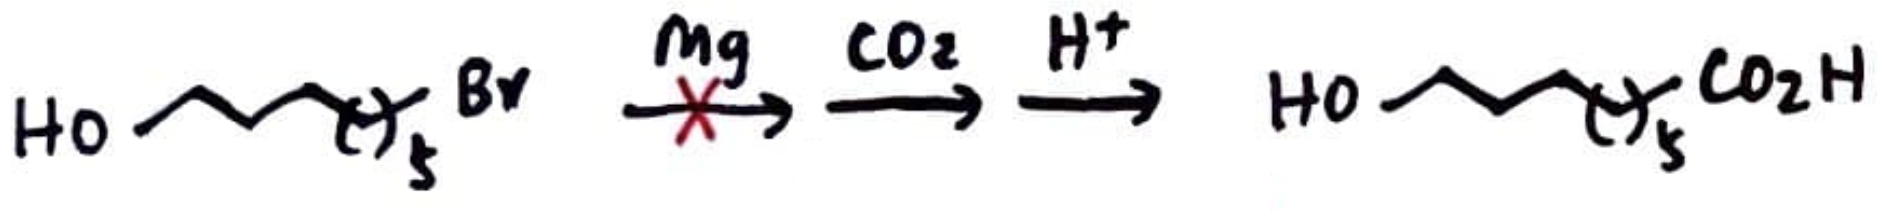
\includegraphics[width=0.5\linewidth]{TTQprobIdentify.png}
        \caption{TTQ: Identify the problem (Grignard with acidic protons).}
        \label{fig:TTQprobIdentify}
    \end{figure}
    \begin{itemize}
        \item We're trying to take an alkyl bromide with magnesium to make a Grignard reagent, which we can then carboxylate and work up into a carboxylic acid.
        \item This won't work because the Grignard intermediate will just deprotonate the acidic alcohol proton.
        \item Remember: Grignards aren't just very strong nucleophiles; they're very strong bases!
    \end{itemize}
    \item TTQ: Fix the problem.
    \begin{figure}[h!]
        \centering
        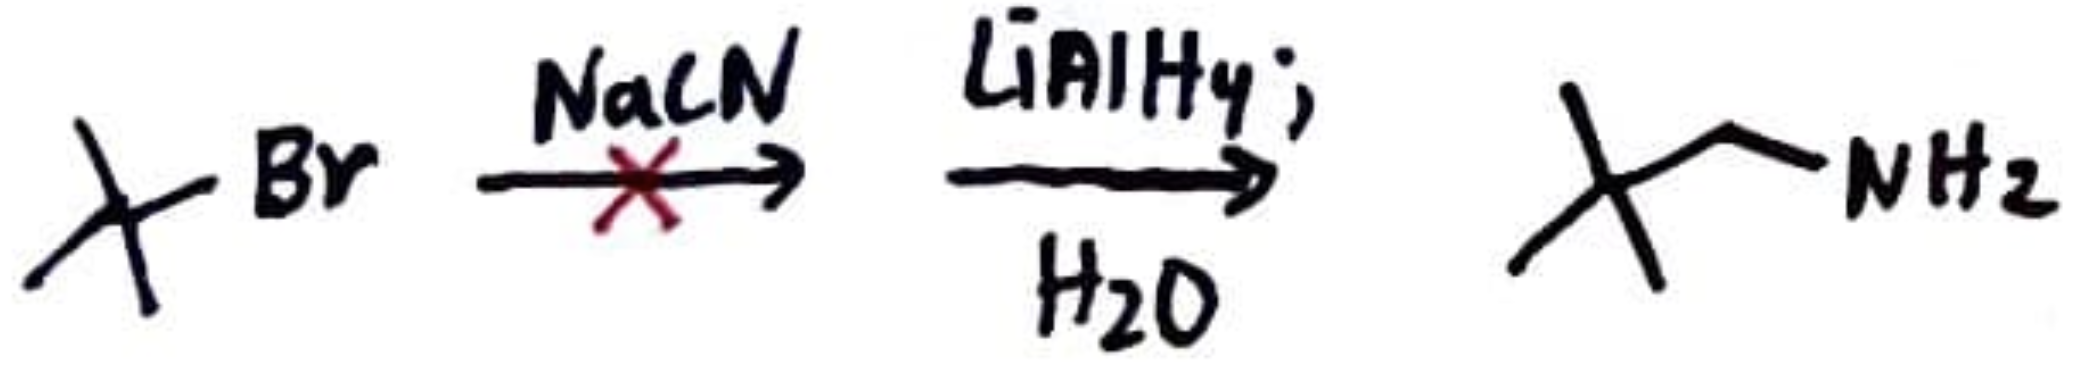
\includegraphics[width=0.4\linewidth]{TTQprobFix2.png}
        \caption{TTQ: Fix the problem (S\textsubscript{N}2 with $3^\circ$).}
        \label{fig:TTQprobFix2}
    \end{figure}
    \begin{itemize}
        \item We do an S\textsubscript{N}2 displacement to form the nitrile, and then reduce to the homologated amine.
        \item Why will this not work?
        \begin{itemize}
            \item Because S\textsubscript{N}2 doesn't happen with $3^\circ$ alkyl halides.
        \end{itemize}
        \item But what if we \emph{have} to convert \emph{tert}-butylbromide to neopentylamine (for example, because someone is holding Prof. Buchwald's cat for ransom)?
        \begin{itemize}
            \item Bromide to Grignard to carboxylic acid to acid chloride to amide to product.
        \end{itemize}
    \end{itemize}
    \item TTQ: Fix the problem.
    \begin{figure}[h!]
        \centering
        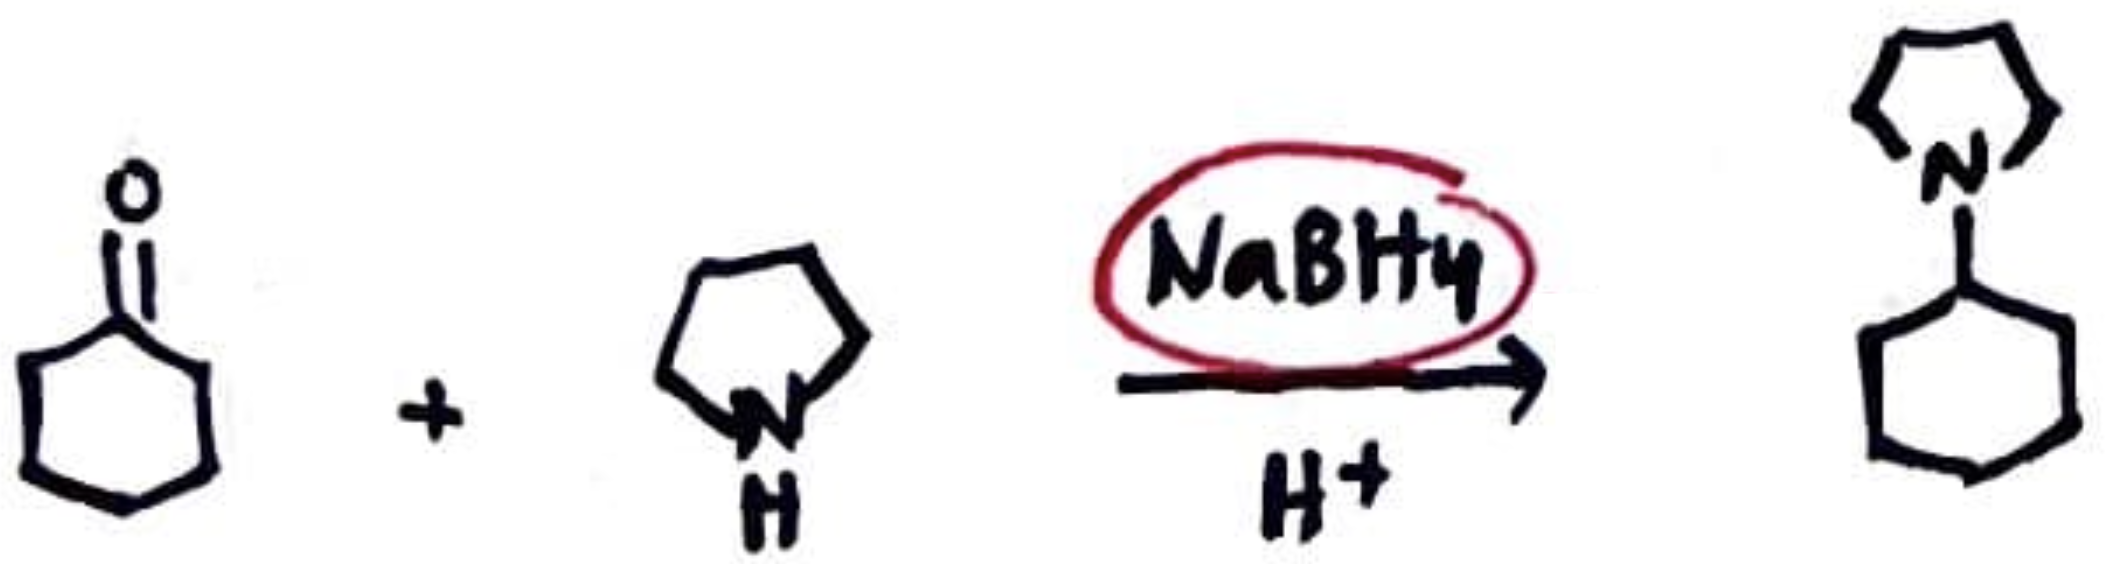
\includegraphics[width=0.4\linewidth]{TTQprobFix3.png}
        \caption{TTQ: Fix the problem (wrong reducing agent).}
        \label{fig:TTQprobFix3}
    \end{figure}
    \pagebreak
    \begin{itemize}
        \item Two reasons this doesn't work.
        \begin{itemize}
            \item \ce{NaBH4} will just reduce the ketone.
            \item \ce{NaBH4} will react with the acid in a nasty way.
        \end{itemize}
        \item We can fix this by using \ce{Na(CN)BH3}.
    \end{itemize}
    \item TTQ: Fix the problem.
    \begin{figure}[h!]
        \centering
        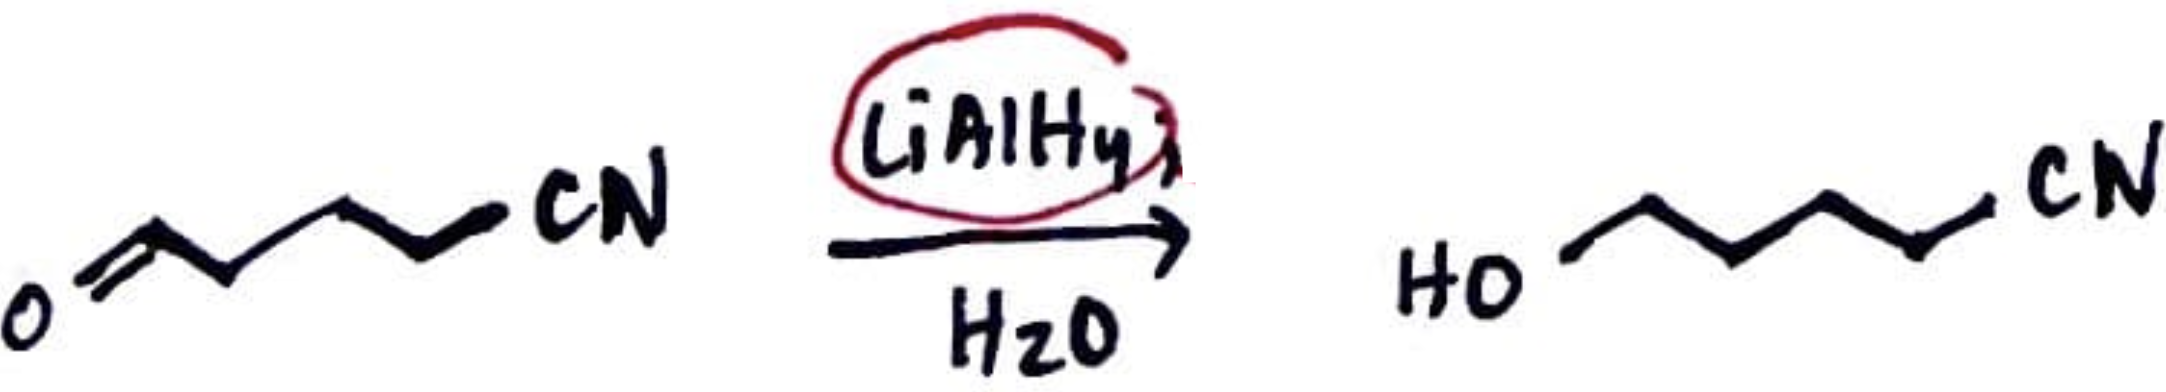
\includegraphics[width=0.4\linewidth]{TTQprobFix4.png}
        \caption{TTQ: Fix the problem (chemoselectivity).}
        \label{fig:TTQprobFix4}
    \end{figure}
    \begin{itemize}
        \item Suppose you want to reduce a cyanoaldehyde to an alcohol.
        \item Why will this not work?
        \begin{itemize}
            \item \ce{LiAlH4} will reduce both.
        \end{itemize}
        \item We can fix this by using \ce{NaBH4}.
    \end{itemize}
    \item TTQ: Fix the problem.
    \begin{figure}[h!]
        \centering
        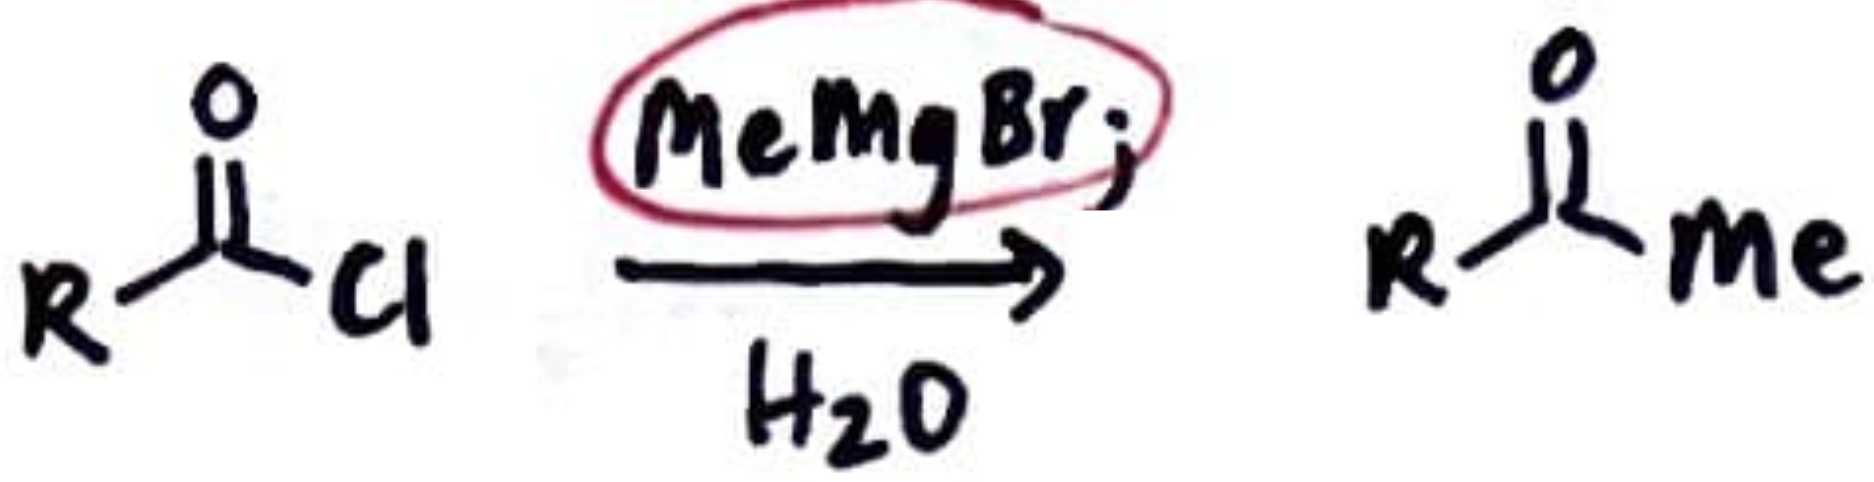
\includegraphics[width=0.3\linewidth]{TTQprobFix5.png}
        \caption{TTQ: Fix the problem (overreactivity).}
        \label{fig:TTQprobFix5}
    \end{figure}
    \begin{itemize}
        \item Treating an acid chloride with methyl magnesium bromide in water gives a methyl ketone.
        \item Why will this not work?
        \begin{itemize}
            \item The Grignard will add twice to afford the tertiary alcohol.
        \end{itemize}
        \item We can fix this with dimethylcopper lithium.
    \end{itemize}
    \item TTQ: Two ways to synthesize a given compound from bromopropane and 1,4-butanediol.
    \begin{figure}[H]
        \centering
        \begin{subfigure}[b]{\linewidth}
            \centering
            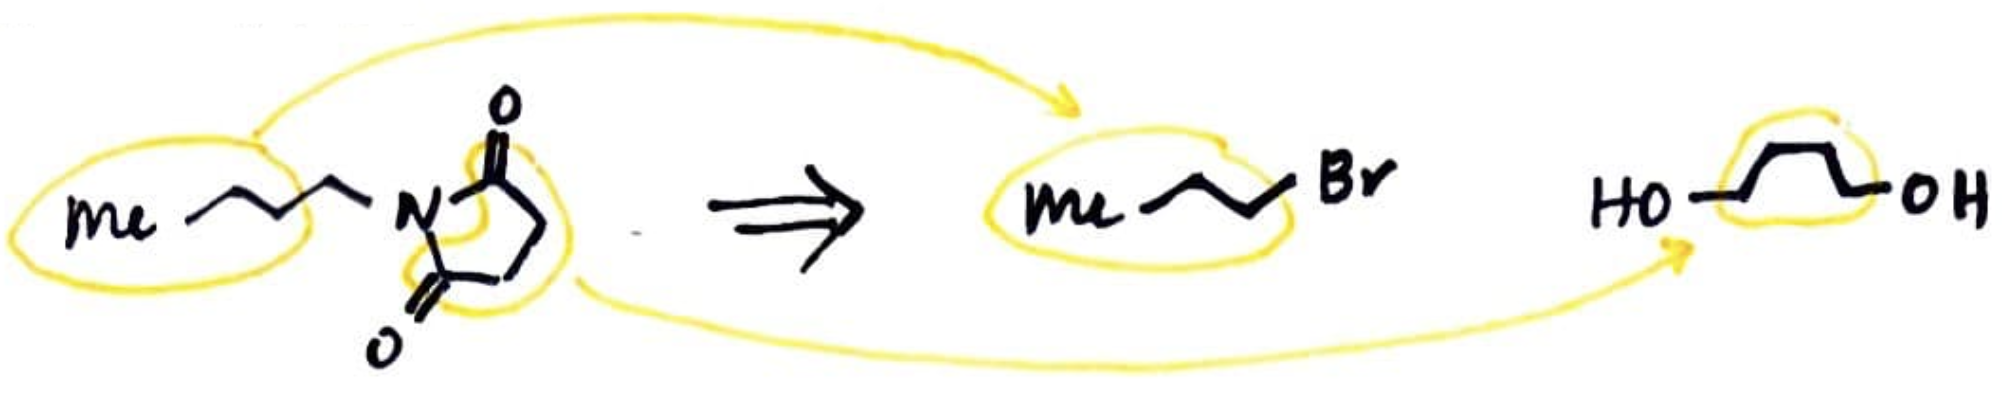
\includegraphics[width=0.55\linewidth]{TTQdiamidea.png}
            \caption{The desired molecule and starting materials.}
            \label{fig:TTQdiamidea}
        \end{subfigure}\\[2em]
        \begin{subfigure}[b]{\linewidth}
            \centering
            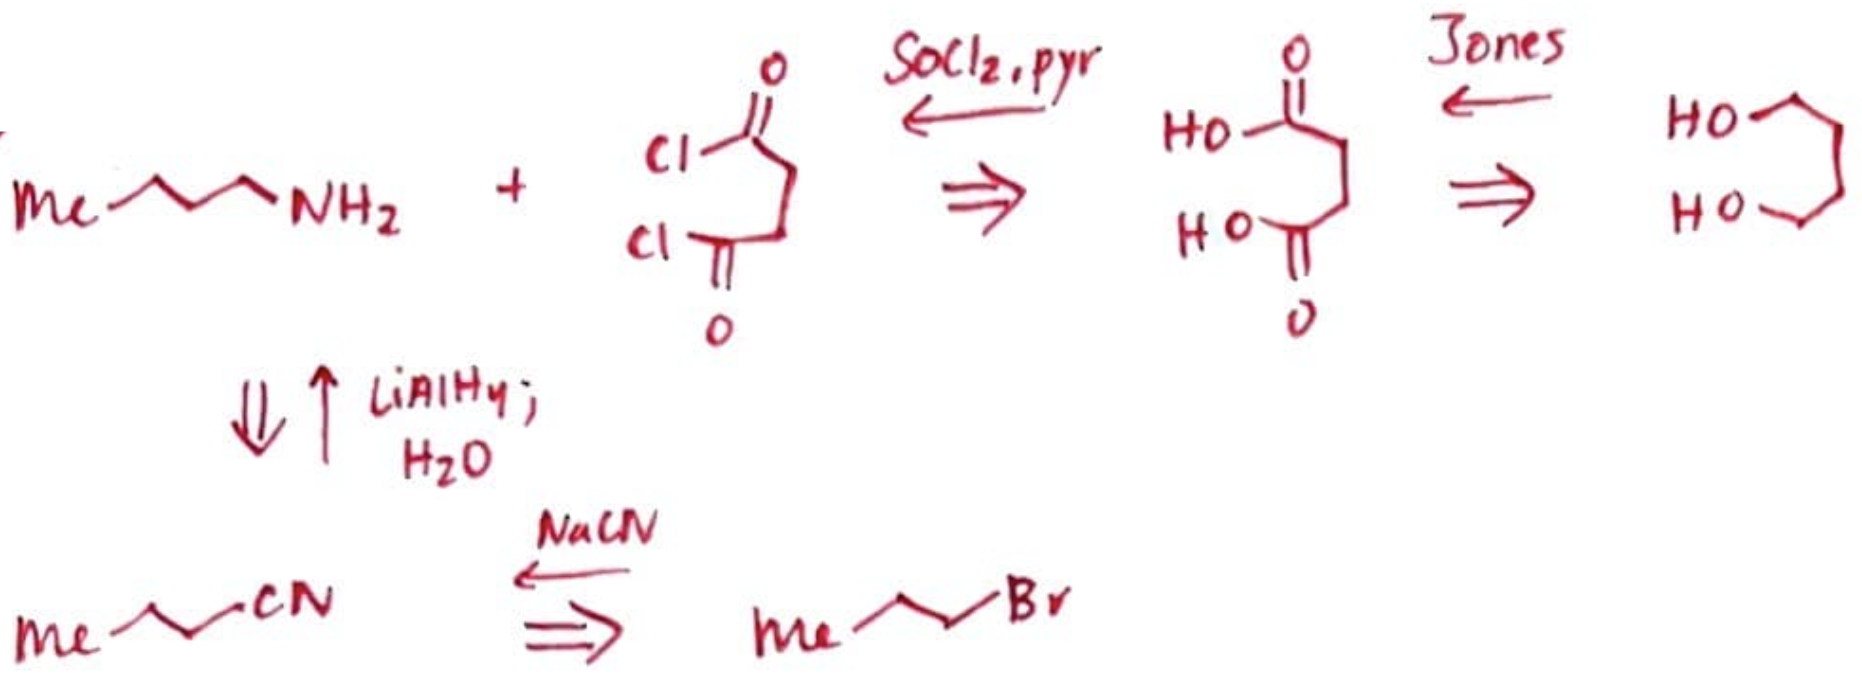
\includegraphics[width=0.6\linewidth]{TTQdiamideb.png}
            \caption{Retrosynthetic pathway.}
            \label{fig:TTQdiamideb}
        \end{subfigure}
        \caption{TTQ: Synthesis of a diamide.}
        \label{fig:TTQdiamide}
    \end{figure}
    \begin{itemize}
        \item First, think about how the carbons might map onto the structure.
        \begin{itemize}
            \item Thus, we need to adjust the oxidation state from alcohol to aldehyde.
            \item We also need to input a \ce{CH2N}.
        \end{itemize}
        \item Easiest way to do this disconnection: Split into a primary amide and a diacetyl chloride (specifically, succinyl chloride).
        \item Let's now retrosynthesize succinyl chloride.
        \begin{itemize}
            \item Next step: Transform succinyl chloride into the dicarboxylic acid via \ce{SOCl2} and \ce{Py}.
            \item Next step: Transform the dicarboxylic acid into the original diol via Jones reagent.
        \end{itemize}
        \item Let's now retrosynthesize the primary amine.
        \begin{itemize}
            \item Next step: Transform the amine into the nitrile via \ce{LiAlH4} followed by \ce{H2O}.
            \item Next step: Transform the nitrile into the original bromopropane via \ce{NaCN}.
        \end{itemize}
        \item Follow up question: Suppose we don't have access to cyanides (as we often don't since they're toxic). How could we go from bromopropane to the primary amine without the cyanide?
        \begin{itemize}
            \item As we just did!
            \item Bromide to Grignard to carboxylic acid to acid chloride to amide to amine.
        \end{itemize}
    \end{itemize}
    \item Could we go directly from the carboxylic acid to the diamide?
    \begin{itemize}
        \item Sure, there are reactions that do this (even though we have not covered them).
        \item But it will be more efficient anyway to go through the acid chloride.
    \end{itemize}
    \item TTQ: Synthesize the given compound from benzene and any compound with less than two carbons.
    \begin{figure}[h!]
        \centering
        \begin{subfigure}[b]{\linewidth}
            \centering
            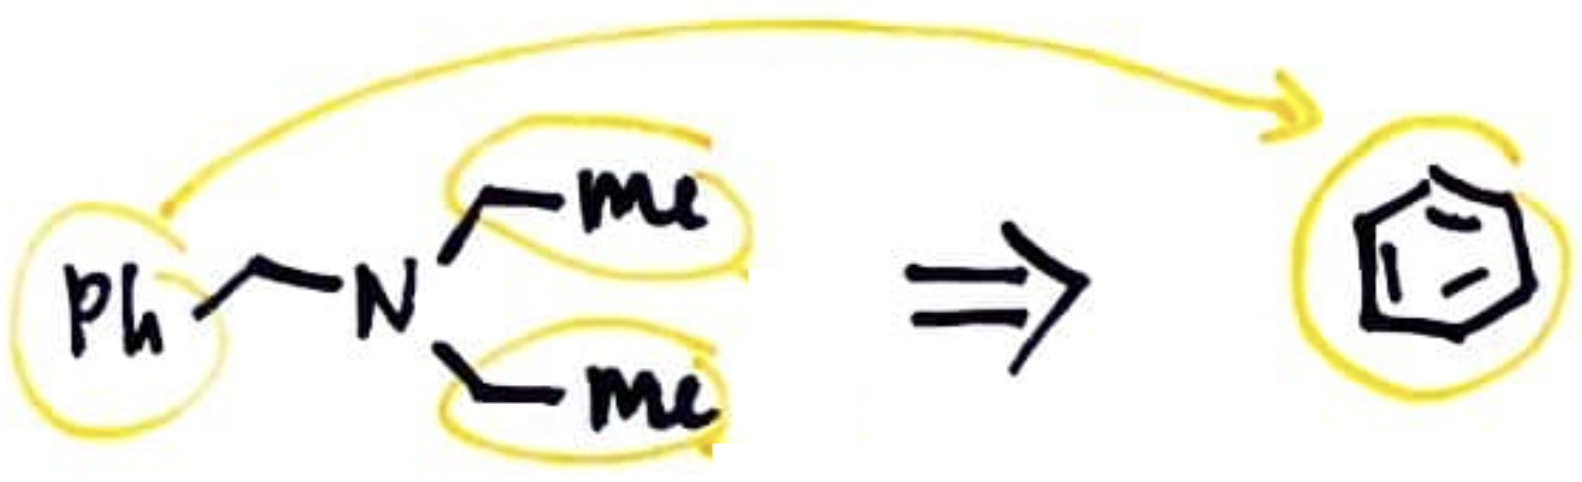
\includegraphics[width=0.35\linewidth]{TTQbenzene2a.png}
            \caption{The desired molecule and starting materials.}
            \label{fig:TTQbenzene2a}
        \end{subfigure}\\[2em]
        \begin{subfigure}[b]{\linewidth}
            \centering
            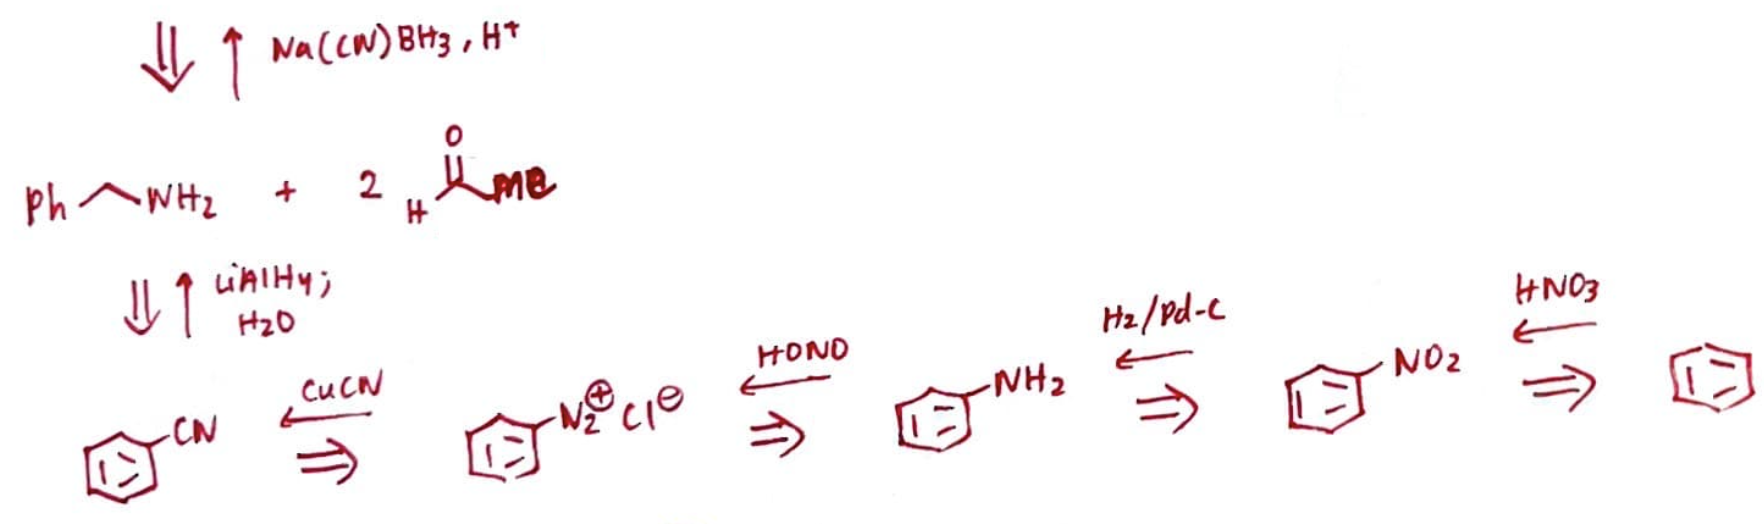
\includegraphics[width=0.9\linewidth]{TTQbenzene2b.png}
            \caption{Retrosynthetic pathway.}
            \label{fig:TTQbenzene2b}
        \end{subfigure}
        \caption{TTQ: Synthesis of a benzene derivative.}
        \label{fig:TTQbenzene2}
    \end{figure}
    \begin{itemize}
        \item First, think about how the carbons might map onto the structure.
        \begin{itemize}
            \item Benzene becomes the phenyl ring.
            \item Each other amine substituent has only two carbons!
        \end{itemize}
        \pagebreak
        \item Transform the product into a primary amine and acetaldehyde (a two-carbon starting material!) via double reductive amination with \ce{Na(CN)BH3} and \ce{H+}.
        \begin{itemize}
            \item Next step: Transform the primary amine into a nitrile via LAH followed by \ce{H2O}.
            \item Next step: Transform the nitrile into an aryl diazonium salt via the Sandmeyer reaction, i.e., \ce{CuCN}.
            \item Next step: Transform the aryl diazonium salt into aniline via HONO.
            \item Next step: Transform aniline into nitrobenzene via \ce{H2} / Pd/C.
            \item Next step: Transform nitrobenzene into benzene via \ce{HNO3}.
        \end{itemize}
        \item Alternate pathway.
        \begin{itemize}
            \item We could retrosynthesize the product to benzaldehyde and diethylamine, and then make both of those.
        \end{itemize}
    \end{itemize}
    \item TTQ: Synthesize the given compound from isobutyramide, a compound we saw last lecture!
    \begin{figure}[h!]
        \centering
        \begin{subfigure}[b]{\linewidth}
            \centering
            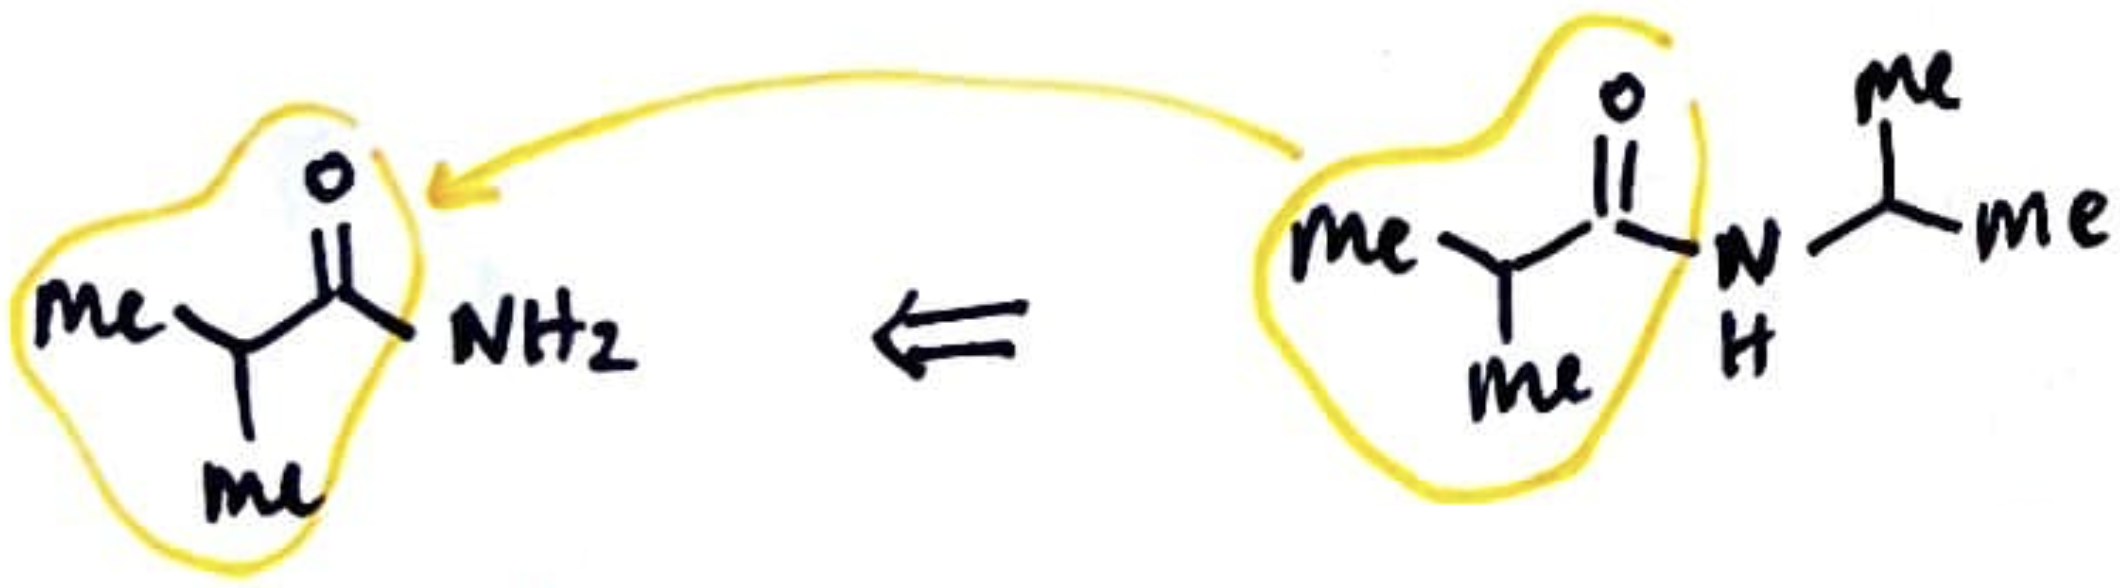
\includegraphics[width=0.45\linewidth]{TTQisobutyramidea.png}
            \caption{The desired molecule and starting materials.}
            \label{fig:TTQisobutyramidea}
        \end{subfigure}\\[2em]
        \begin{subfigure}[b]{\linewidth}
            \centering
            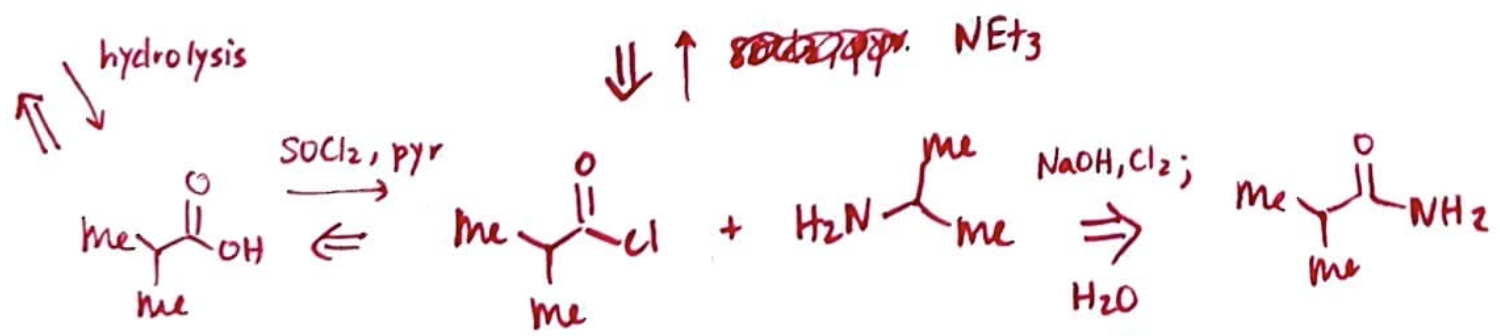
\includegraphics[width=0.75\linewidth]{TTQisobutyramideb.png}
            \caption{Retrosynthetic pathway.}
            \label{fig:TTQisobutyramideb}
        \end{subfigure}
        \caption{TTQ: Synthesis of a pseudodimer of isobutyramide.}
        \label{fig:TTQisobutyramide}
    \end{figure}
    \begin{itemize}
        \item Transform the product into an acid chloride and a primary amine.
        \item Let's now retrosynthesize the acid chloride.
        \begin{itemize}
            \item Next step: Transform the acid chloride into the carboxylic acid via \ce{SOCl2} and \ce{Py}.
            \item Next step: Transform the carboxylic acid into isobutyramide via amide hydrolysis, i.e., \ce{H3O+}.
        \end{itemize}
        \item Let's now retrosynthesize the primary amine.
        \begin{itemize}
            \item Next step: Transform the amine into the starting material via the Hofmann rearrangement, i.e., \ce{NaOH}, \ce{Cl2}, and \ce{H2O}.
        \end{itemize}
    \end{itemize}
    \item Prof. Buchwald reviews the mechanism of the Hofmann rearrangement.
    \item TTQ: Synthesize the compound shown in Figure \ref{fig:TTQstereoa}.
    \begin{figure}[h!]
        \centering
        \begin{subfigure}[b]{\linewidth}
            \centering
            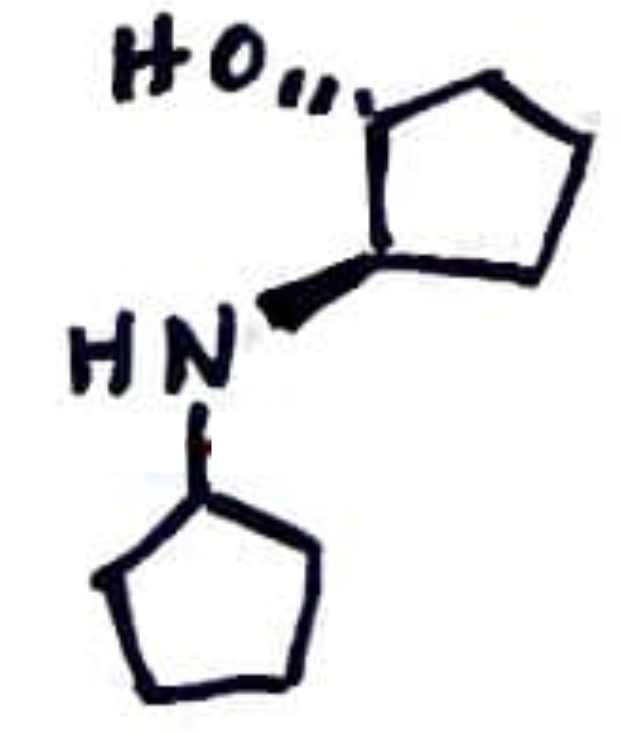
\includegraphics[width=0.1\linewidth]{TTQstereoa.png}
            \caption{The desired molecule.}
            \label{fig:TTQstereoa}
        \end{subfigure}\\[2em]
        \begin{subfigure}[b]{\linewidth}
            \centering
            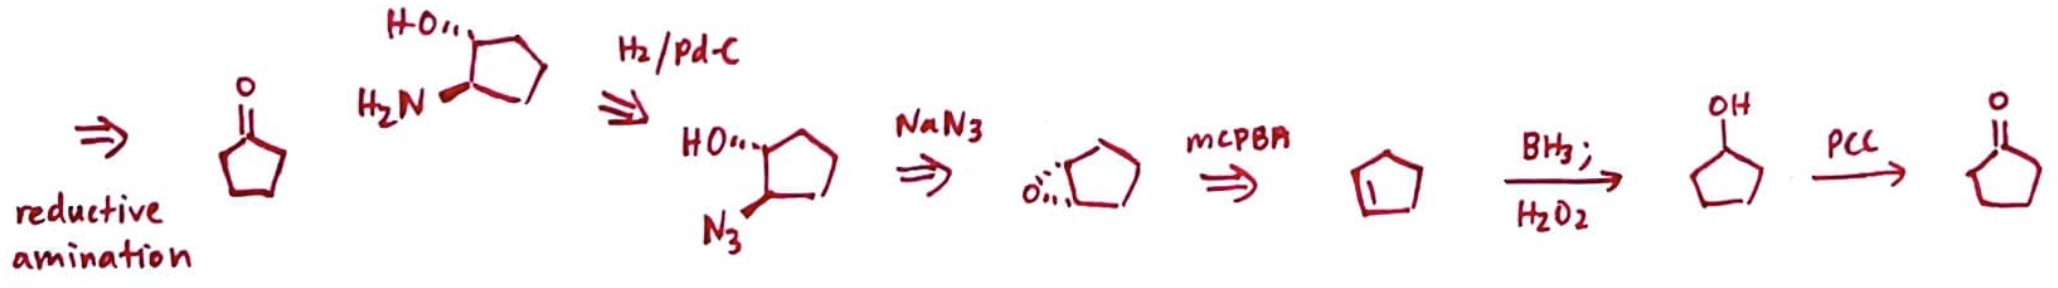
\includegraphics[width=0.95\linewidth]{TTQstereob.png}
            \caption{Retrosynthetic pathway.}
            \label{fig:TTQstereob}
        \end{subfigure}
        \caption{TTQ: Synthesis involving stereochemistry.}
        \label{fig:TTQstereo}
    \end{figure}
    \begin{itemize}
        \item Running out of time, so Prof. Buchwald gives an outline of the solution to this problem.
        \item Transform the product into an imine via \ce{NaBH4}.
        \begin{itemize}
            \item Next step: Transform the imine into cyclopentanone and an aminoalcohol.
            \item Next step: Transform the \emph{trans}-1,2-aminoalcohol into an epoxide as in the upper pathway of Figure \ref{fig:aminoalcoholEpox}.
        \end{itemize}
        \item Cyclohexanone could have come from cyclohexene via hydroboration followed by PCC.
    \end{itemize}
    \item Final pieces of advice.
    \begin{itemize}
        \item Do everything backwards slowly, step by step. Don't skip any! It will just confuse you.
        \item Take some time to study --- that will help you on the exam!
        \item Take some time to relax --- that will help you on the exam!
        \item Don't forget to write your review cards.
    \end{itemize}
\end{itemize}




\end{document}